\documentclass[12pt]{article}

\usepackage{graphicx}
\graphicspath{{images/}}
\usepackage{hyperref}
\hypersetup{colorlinks=true, citecolor=red, linkcolor=black, urlcolor=blue}
%\usepackage[duipsnames]{xcolor}
%\usepackage{caption}
\usepackage{subcaption}
\usepackage{apacite}





\title{Internship Report\\On\\“Web \& App Development\\@\\The Sparks Foundation - Singapore”}
\author{Rishav Pandey\\Senior Undergraduate @ Jabalpur Engineering College}
\date{}

\begin{document}
\maketitle
\clearpage
\tableofcontents
\clearpage
\listoffigures
\clearpage

\section[Certificate Of Selection]{\underline{Certificate Of Selection}}
\begin{figure}[h]
\centering

\includegraphics[scale=0.4]{1642006136608.png}
\caption{Selection Certificate}
\end{figure}
\clearpage

\section[Certificate Of Internship Completion]{\underline{Certificate Of Internship Completion}}
\begin{figure}[h]
\centering

\includegraphics[scale=0.4]{1642006136604.png}
\caption{Internship Certificate}
\end{figure}
\clearpage

\section[Recommendation Letter from the\\ Managing Director of TSF, Singapore\\ for outstanding performance in GRIP]{\underline{Recommendation Letter from the}\\\underline{Managing Director of TSF, Singapore}\\\underline{for outstanding performance in GRIP}}
\begin{figure}[h]
\centering

\includegraphics[scale=0.375]{1642006136598.png}
\caption{Recommendation Letter}
\end{figure}
\clearpage

\section{The Sparks Foundation}
Sparks Foundation is a Singapore based IT company. It runs a Graduate Rotational Internship Programme every year. In this internship programme they hire STEM students for technical tasks.\\

In the month of May’21, I got selected to work as a \textbf{Web \& App\\ Development Intern} for one month. Tasks which I completed during my entire tenure are summarized below:

\subsection{Task 1: Payment Gateway Integration}
\begin{itemize}
\item Create a simple website where payment gateway is integrated.
\item There will be a simple donate button on homepage. On clicking the donate button, the user will land on the payment page where user can select the amount to be paid and the payment type, e.g. credit card, Paypal, etc.
\item Once the payment is done and invoice will be generated and email will be sent to the user for the payment received. The invoice will contain the amount.
\item On any page / email, only basic information is needed.
\item Create your own temporary / sandbox / testing accounts with 3rd party for integrations.
\item Host the website at 000webhost, github.io, heroku app or any other free hosting provider. Check in code in gitlab.

\end{itemize}


\subsection{Task 2: Social Media Integration}
\begin{itemize}
\item Create a mobile app, where user can login through at least two social media from such as Facebook and Google.
\item After login, display all the details (e.g. Name, profile photo, email, etc.) on the second page.
\item Take help of online tutorials and You tube videos.
\item No backend / server-side programming required.
\item Very good-looking UI and responsive UI, which should work for mobiles as well as tablets.
\item Clean code is a must.
\item Upload video demo of your application on you tube and submit the url.
\end{itemize}

\subsection{Task 3: CI/CD: Cloud Computing}
\begin{itemize}
\item Read up about AWS or Azure.
\item Write up about the steps of setup and essentials of AWS EC2 or Azure VM (one page step by step).
\item Create an EC2 or azure VM instance and access it through ssh from your pc over internet.
\item In the EC2, deploy and run any application (a website with tomcat/spring boot) or python-based project.
\item Use at least one service apart from EC2 or VM, i.e. Database service, or MQ, ML, Mobile or any other services provided by AWS or Azure.
\item Submit the URL of the application which is running on EC2.
\item Your video should show that you are able to run applications on cloud.
\end{itemize}
\clearpage

\section{Works Carried Out In Task 1:}
Designed an animal donation website named 'Saving Paws' and then integrated a payment gateway page in it. There is a donate button on home page, just by tapping the same user is directed to the payment page. Once the payment is done, an invoice is generated and email is sent to the user for the payment received. The invoice contains the amount. [Figure \ref{Untitled1.png}, \ref{Untitled3.png}, \ref{Untitled4.png}, \ref{Untitled5.png}]

\subsection{Home Page:}
\begin{figure}[h]
\centering
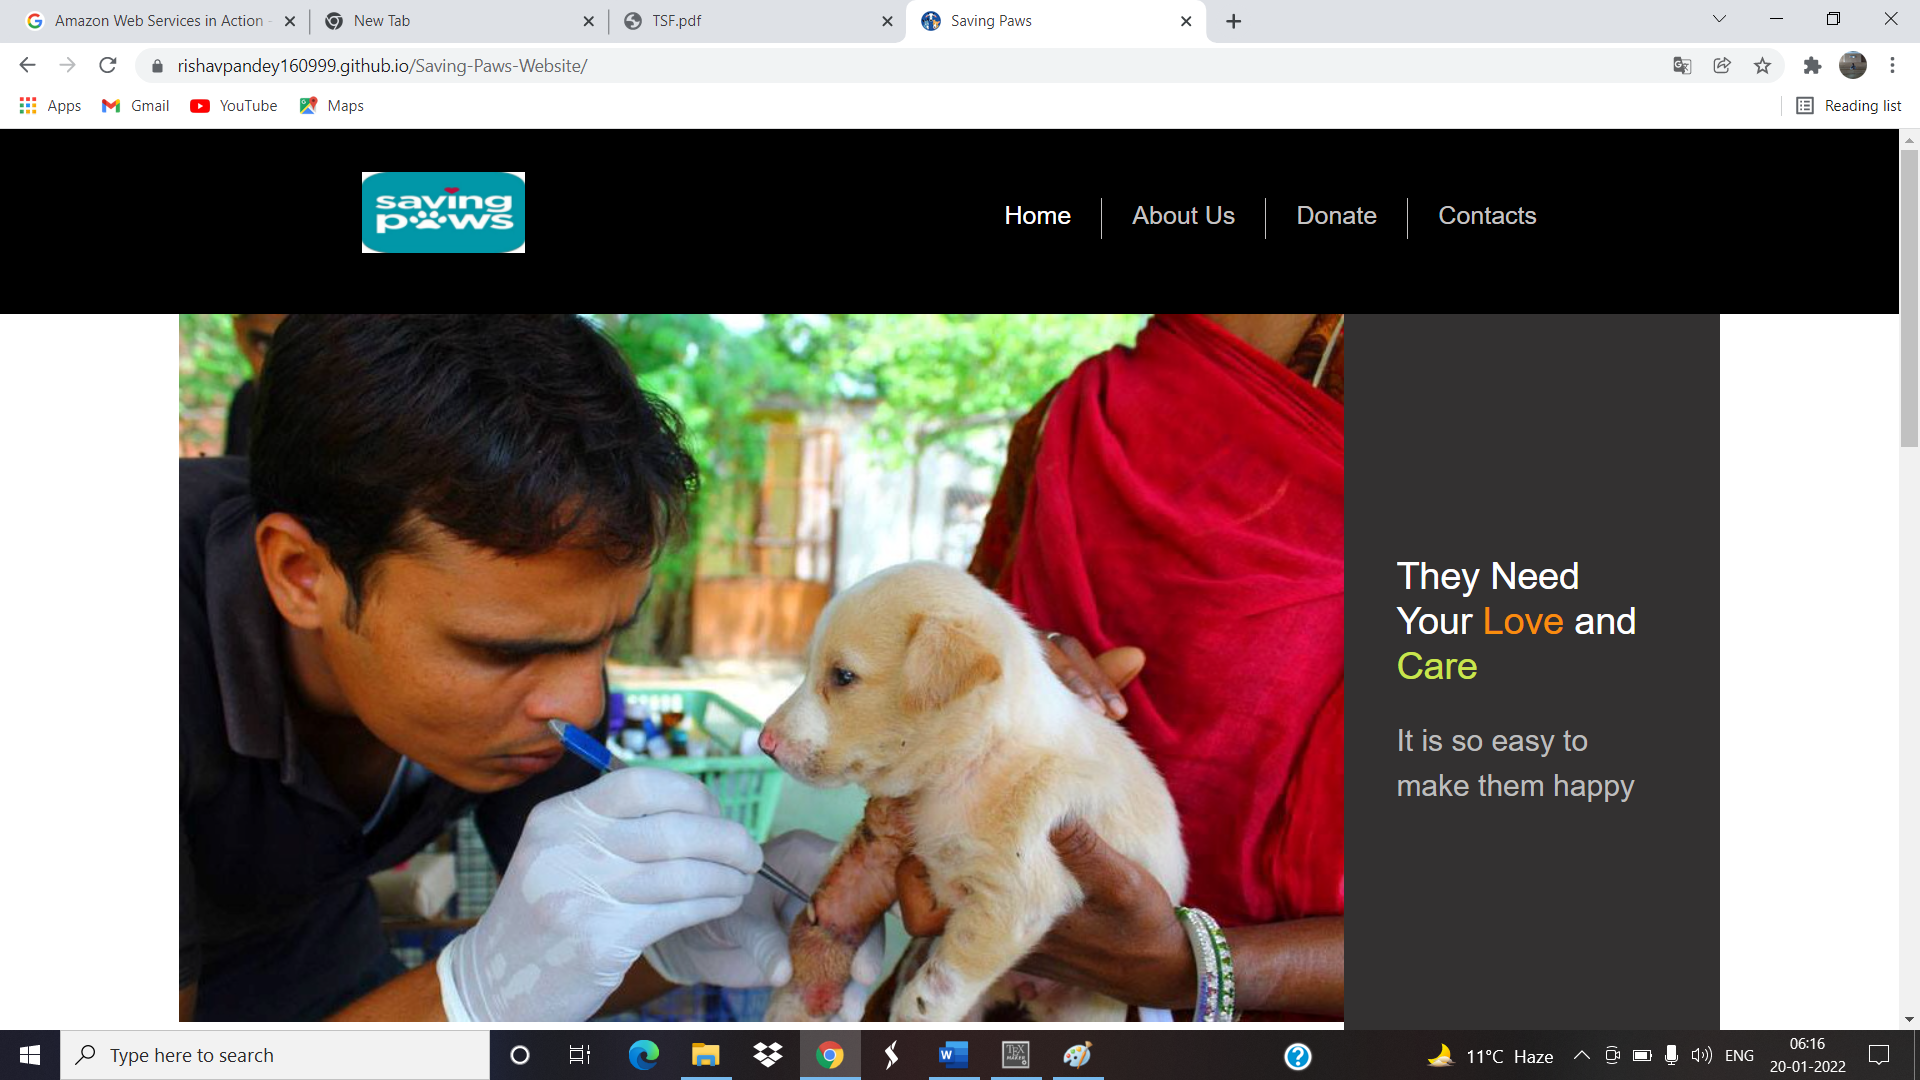
\includegraphics[scale=0.23]{Untitled1.png}
\caption{Home Page (i)}
\label{Untitled1.png}
\end{figure}


\begin{figure}[h]
\centering
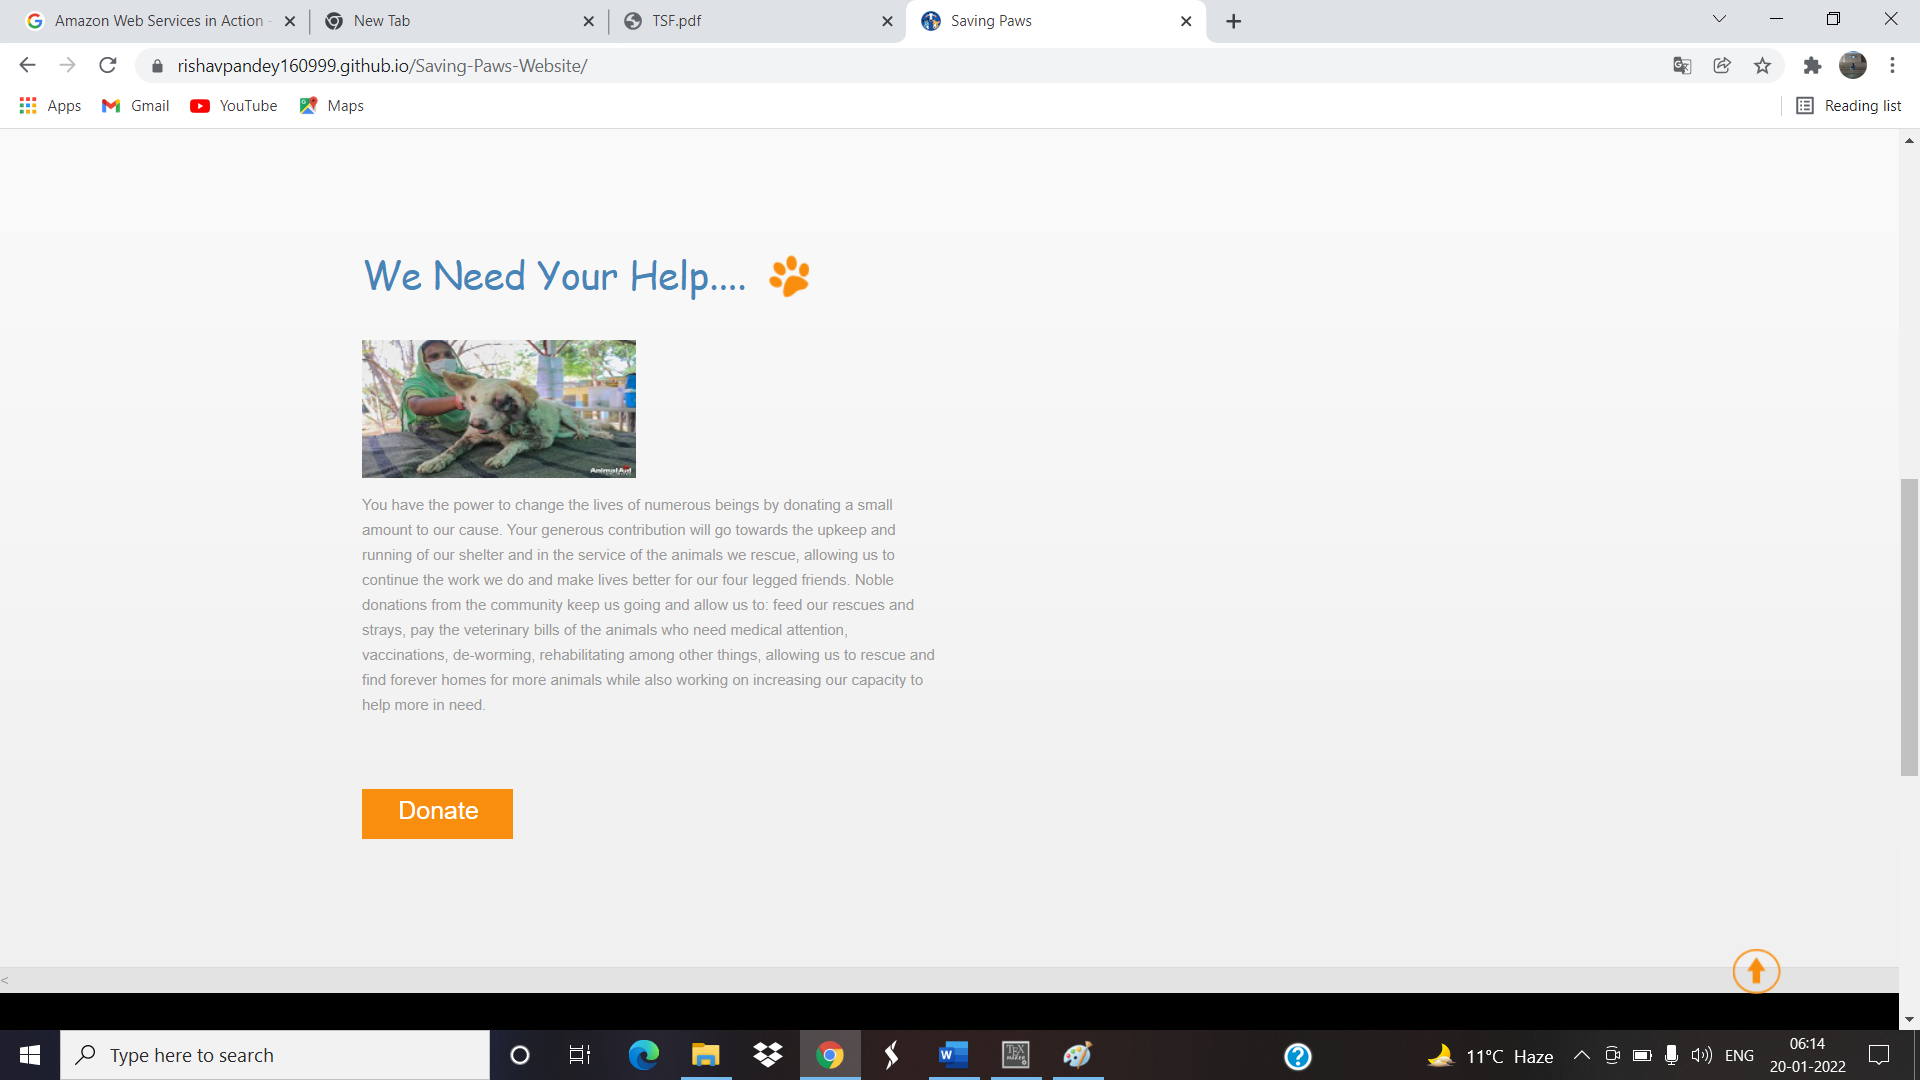
\includegraphics[scale=0.23]{Untitled.png}
\caption{Home Page (ii)}
\label{Untitled.png}
\end{figure}
\clearpage

\begin{figure}[h]
\centering
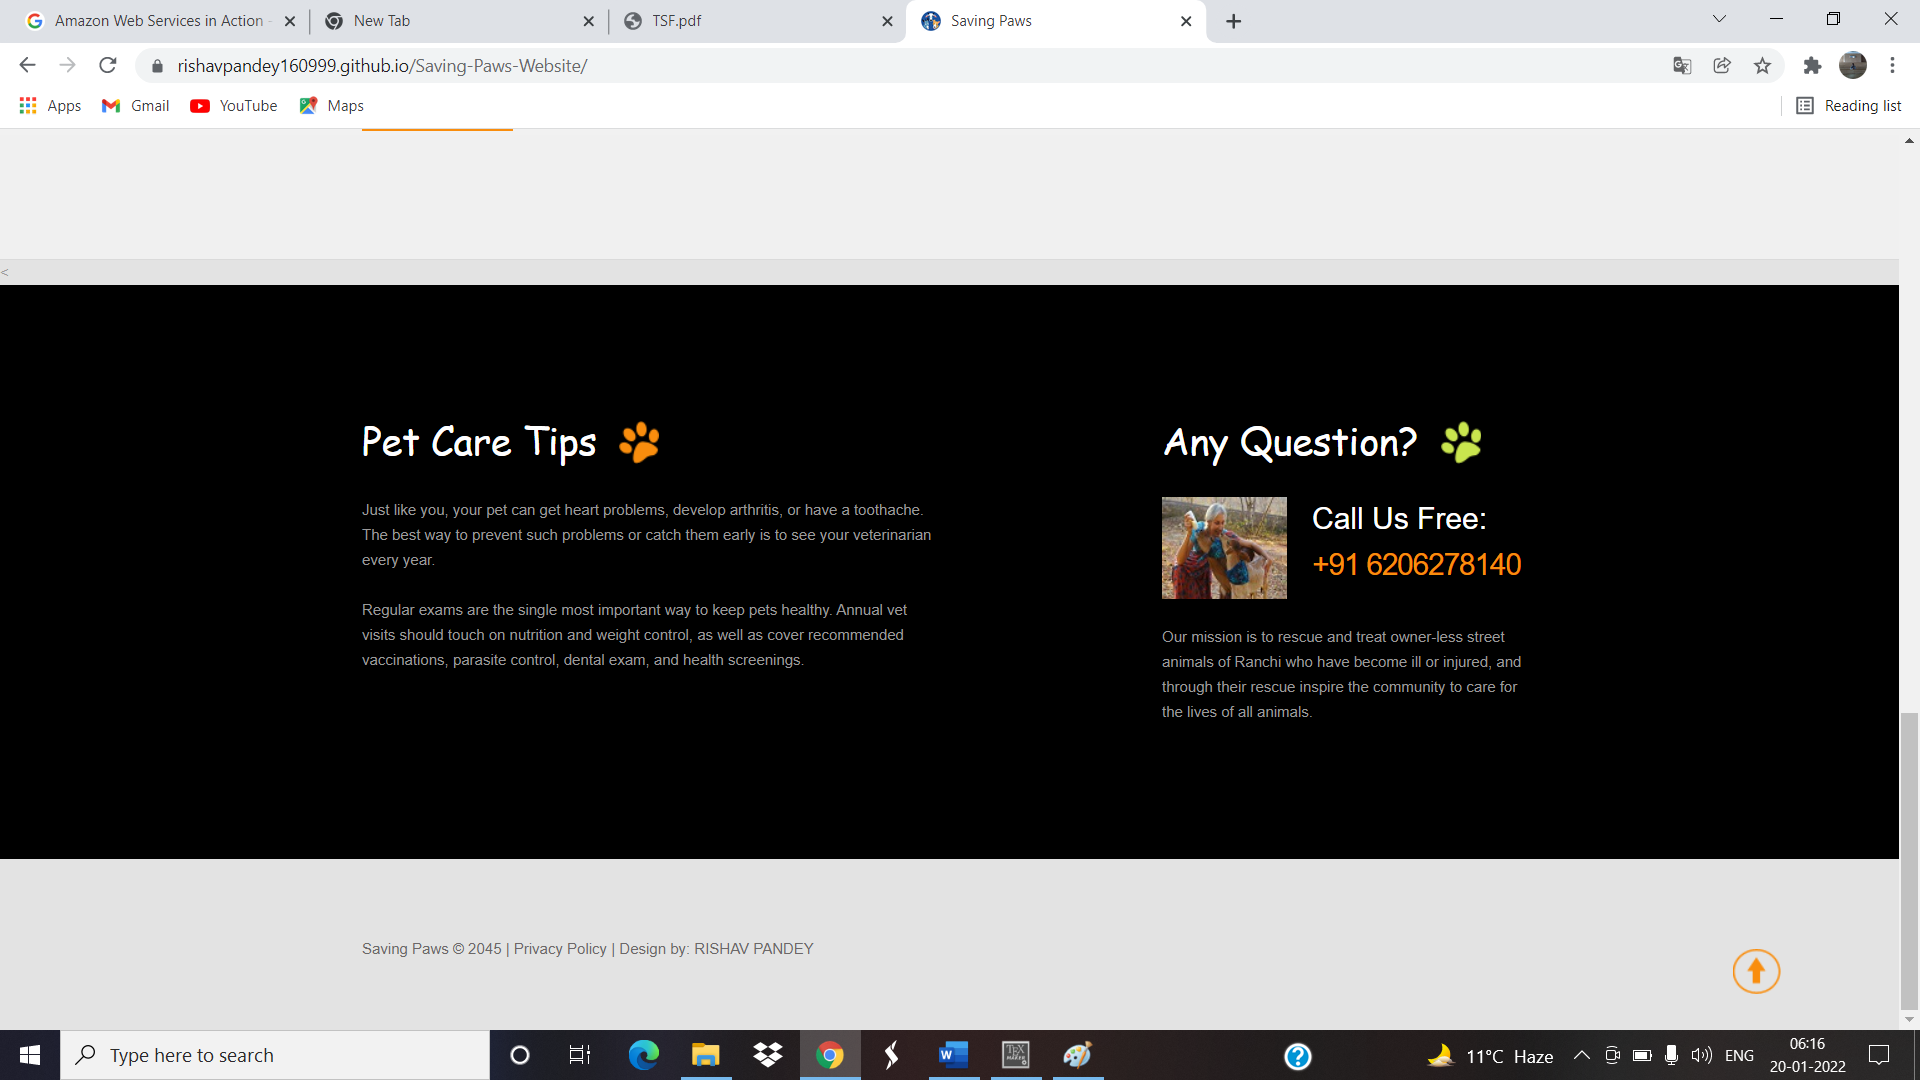
\includegraphics[scale=0.26]{Untitled2.png}
\caption{Home Page (iii)}
\label{Untitled2.png}
\end{figure}


\subsection{About Us Page:}
\begin{figure}[h]
\centering
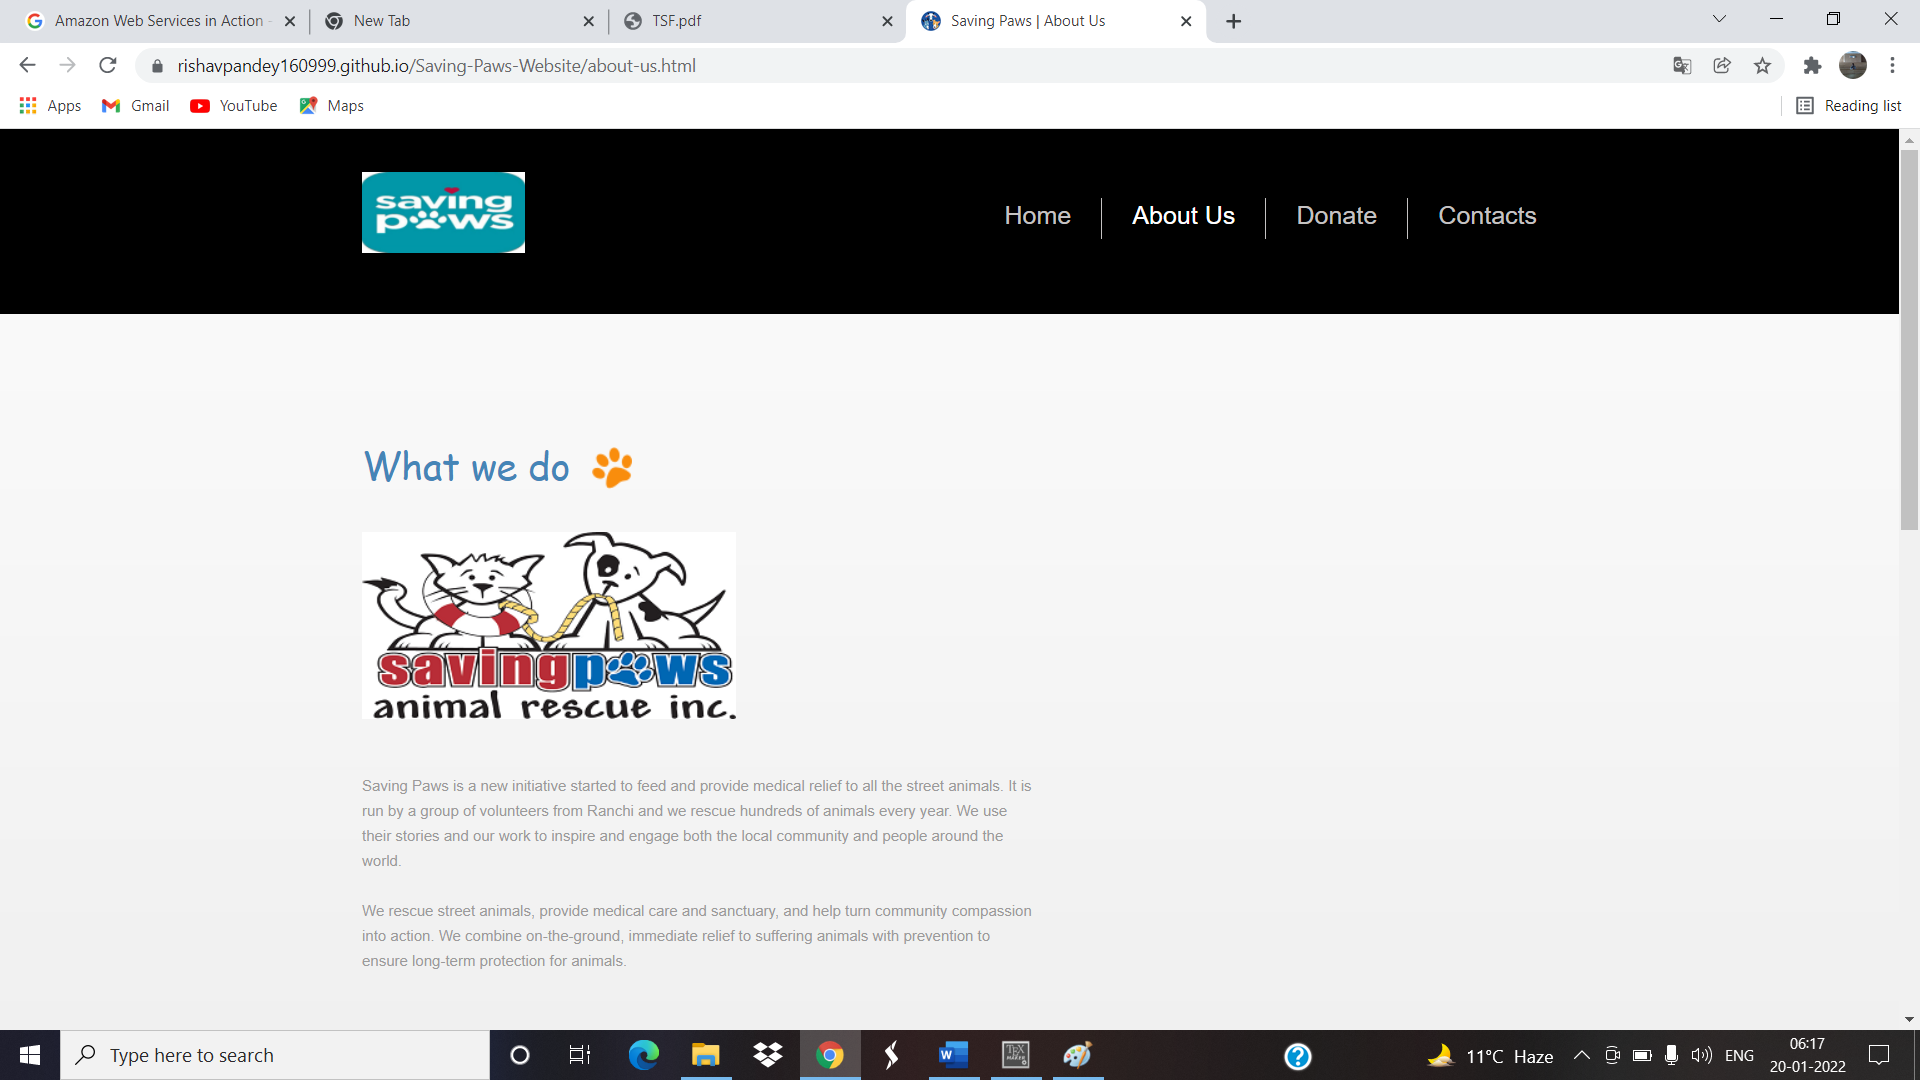
\includegraphics[scale=0.26]{Untitled3.png}
\caption{About Us Page}
\label{Untitled3.png}
\end{figure}
\clearpage

\subsection{Donate Page:}
\begin{figure}[h]
\centering
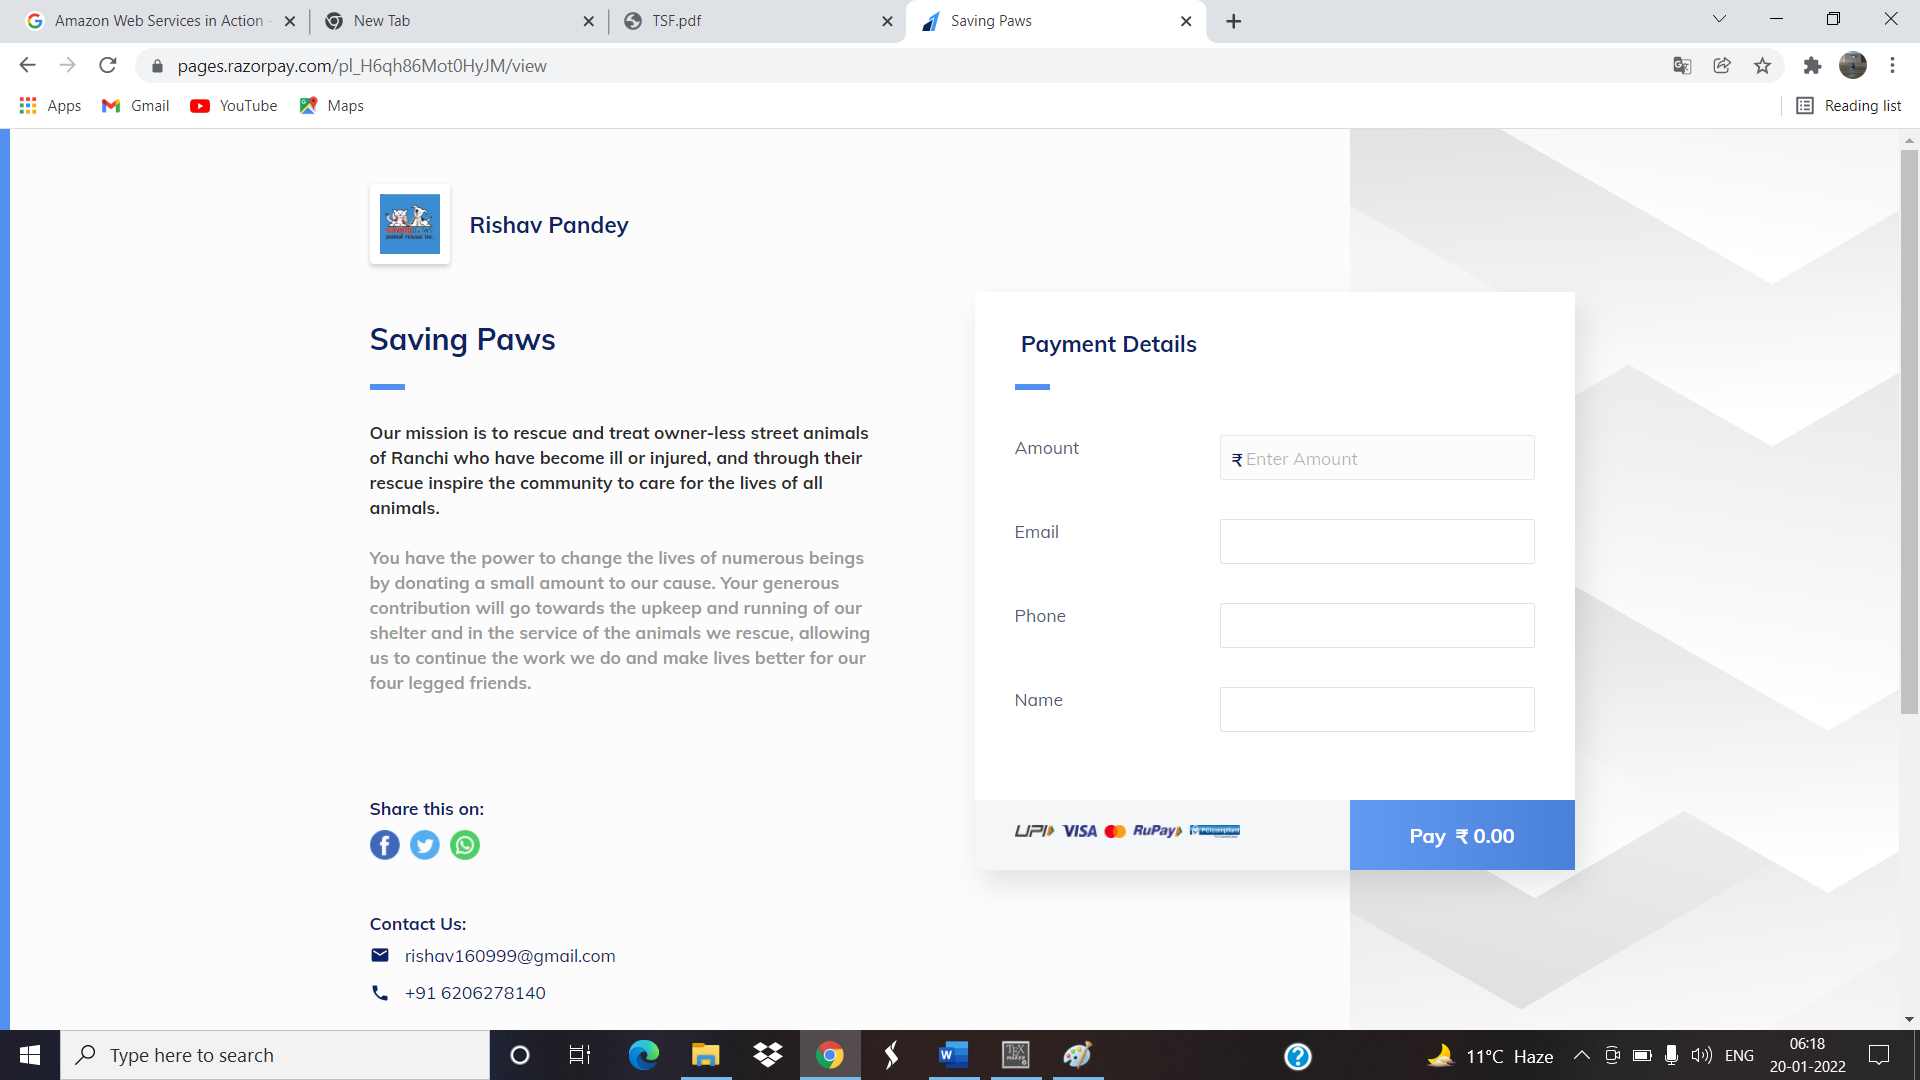
\includegraphics[scale=0.23]{Untitled4.png}
\caption{Donate Page}
\label{Untitled4.png}
\end{figure}



\subsection{Contact Us Page:}
\begin{figure}[h]
\centering
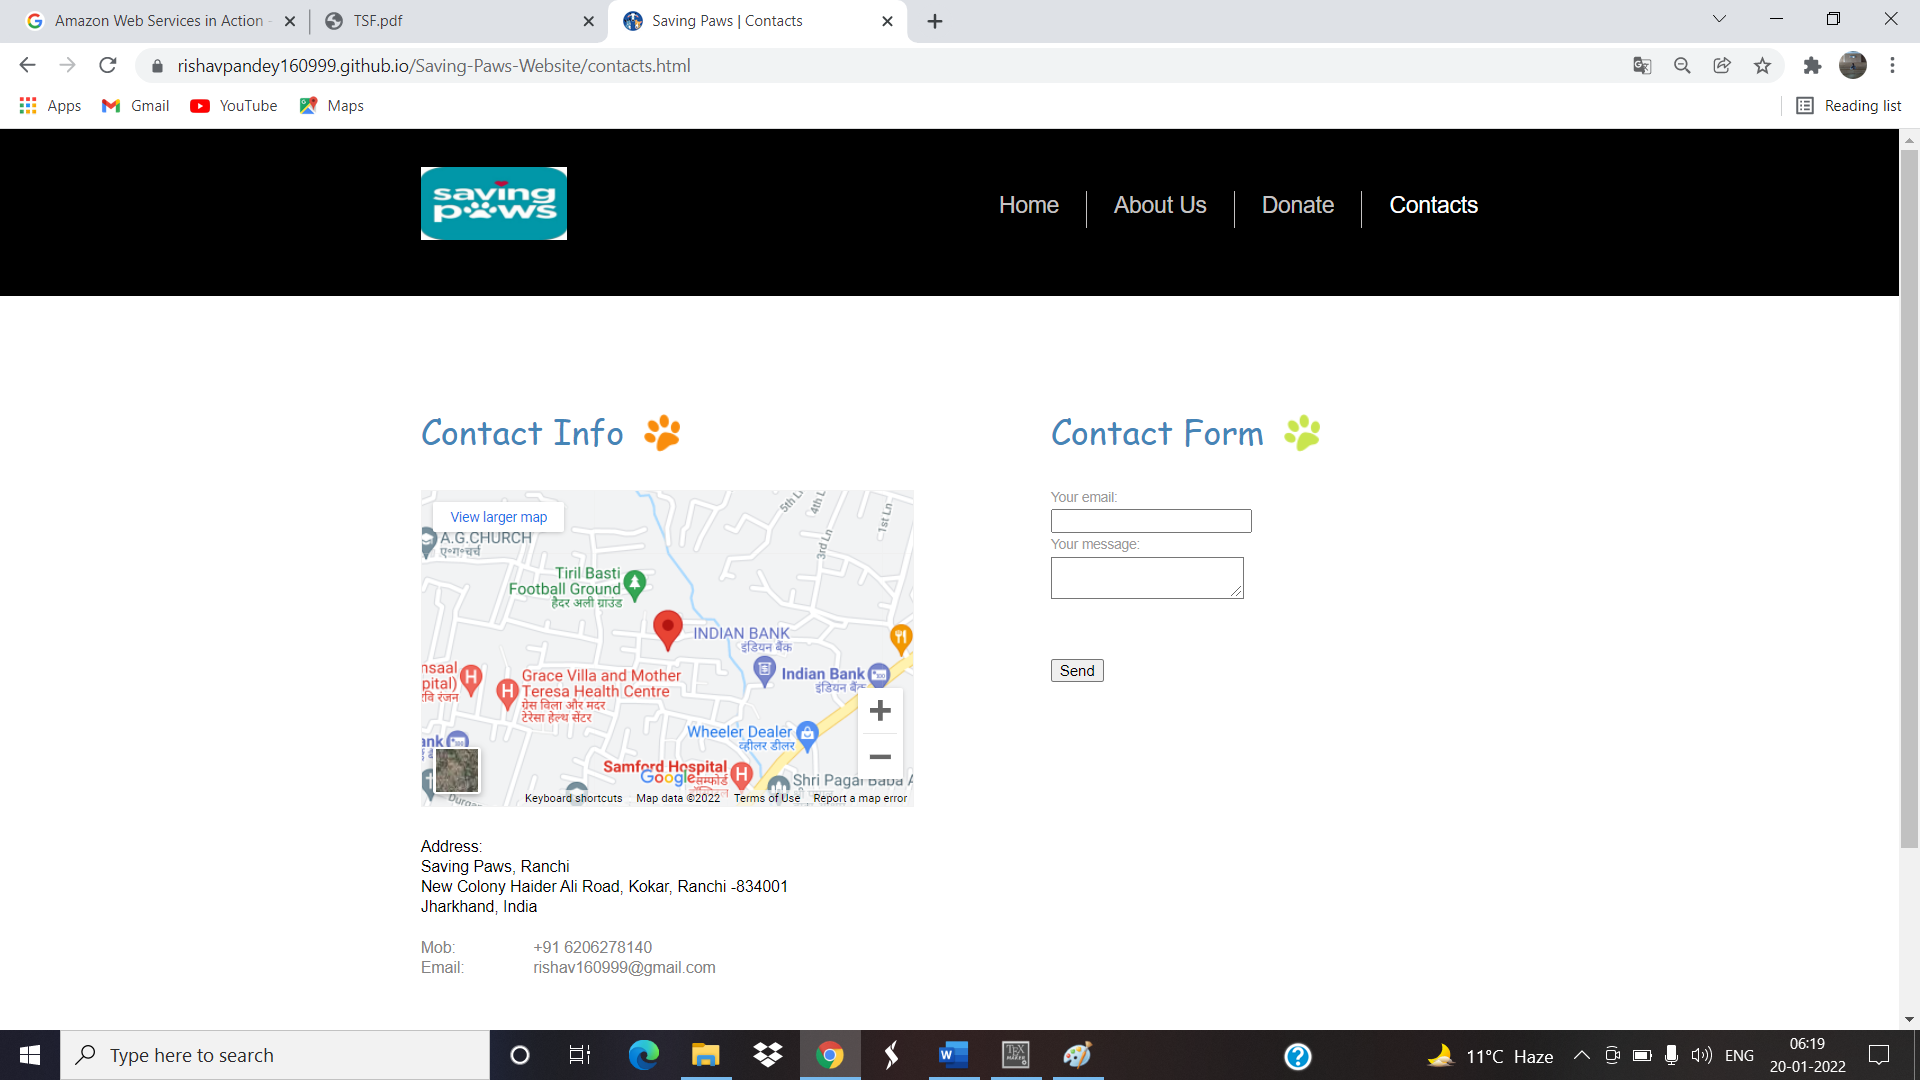
\includegraphics[scale=0.23]{Untitled5.png}
\caption{Contact Us Page}
\label{Untitled5.png}
\end{figure}





\href{https://rishavpandey160999.github.io/Saving-Paws-Website/}{Link of the website}\\

\href{https://github.com/rishavpandey160999/Saving-Paws-Website}{GitHub Repo}\\

\href{https://youtu.be/sJ11fdcWGwQ}{Presentation}
\clearpage

\section{Works Carried Out In Task 2:}
Designed an android app named "Euro 2 INR Converter" which converts a given amount in Euro into INR. For creating the same I used JAVA and tool like Android Studio. I've integrated Google and Facebook Sign-in in it, so that a user can sign in by any of the two ways. Once the user is signed in, their name, email, and profile picture is displayed on the next screen. User can further continue to the next interface i.e. "Euro 2 INR Converter" page. [Figure \ref{Splash Screen}, \ref{SignIn Page}, \ref{Profile Page}, \ref{Euro 2 INR Convertor Page}]

\subsection{Splash Screen:}

\begin{figure}[h]
\centering

\includegraphics[scale=0.13]{146977618-085ec667-1e42-416a-87fb-1c32954f3d3f.jpg}
\caption{Splash Screen}
\label{Splash Screen}
\end{figure}
\clearpage

\subsection{Sign-in Page:}
\begin{figure}[h]
\centering
\begin{subfigure}[h]{0.3\textwidth}
\centering
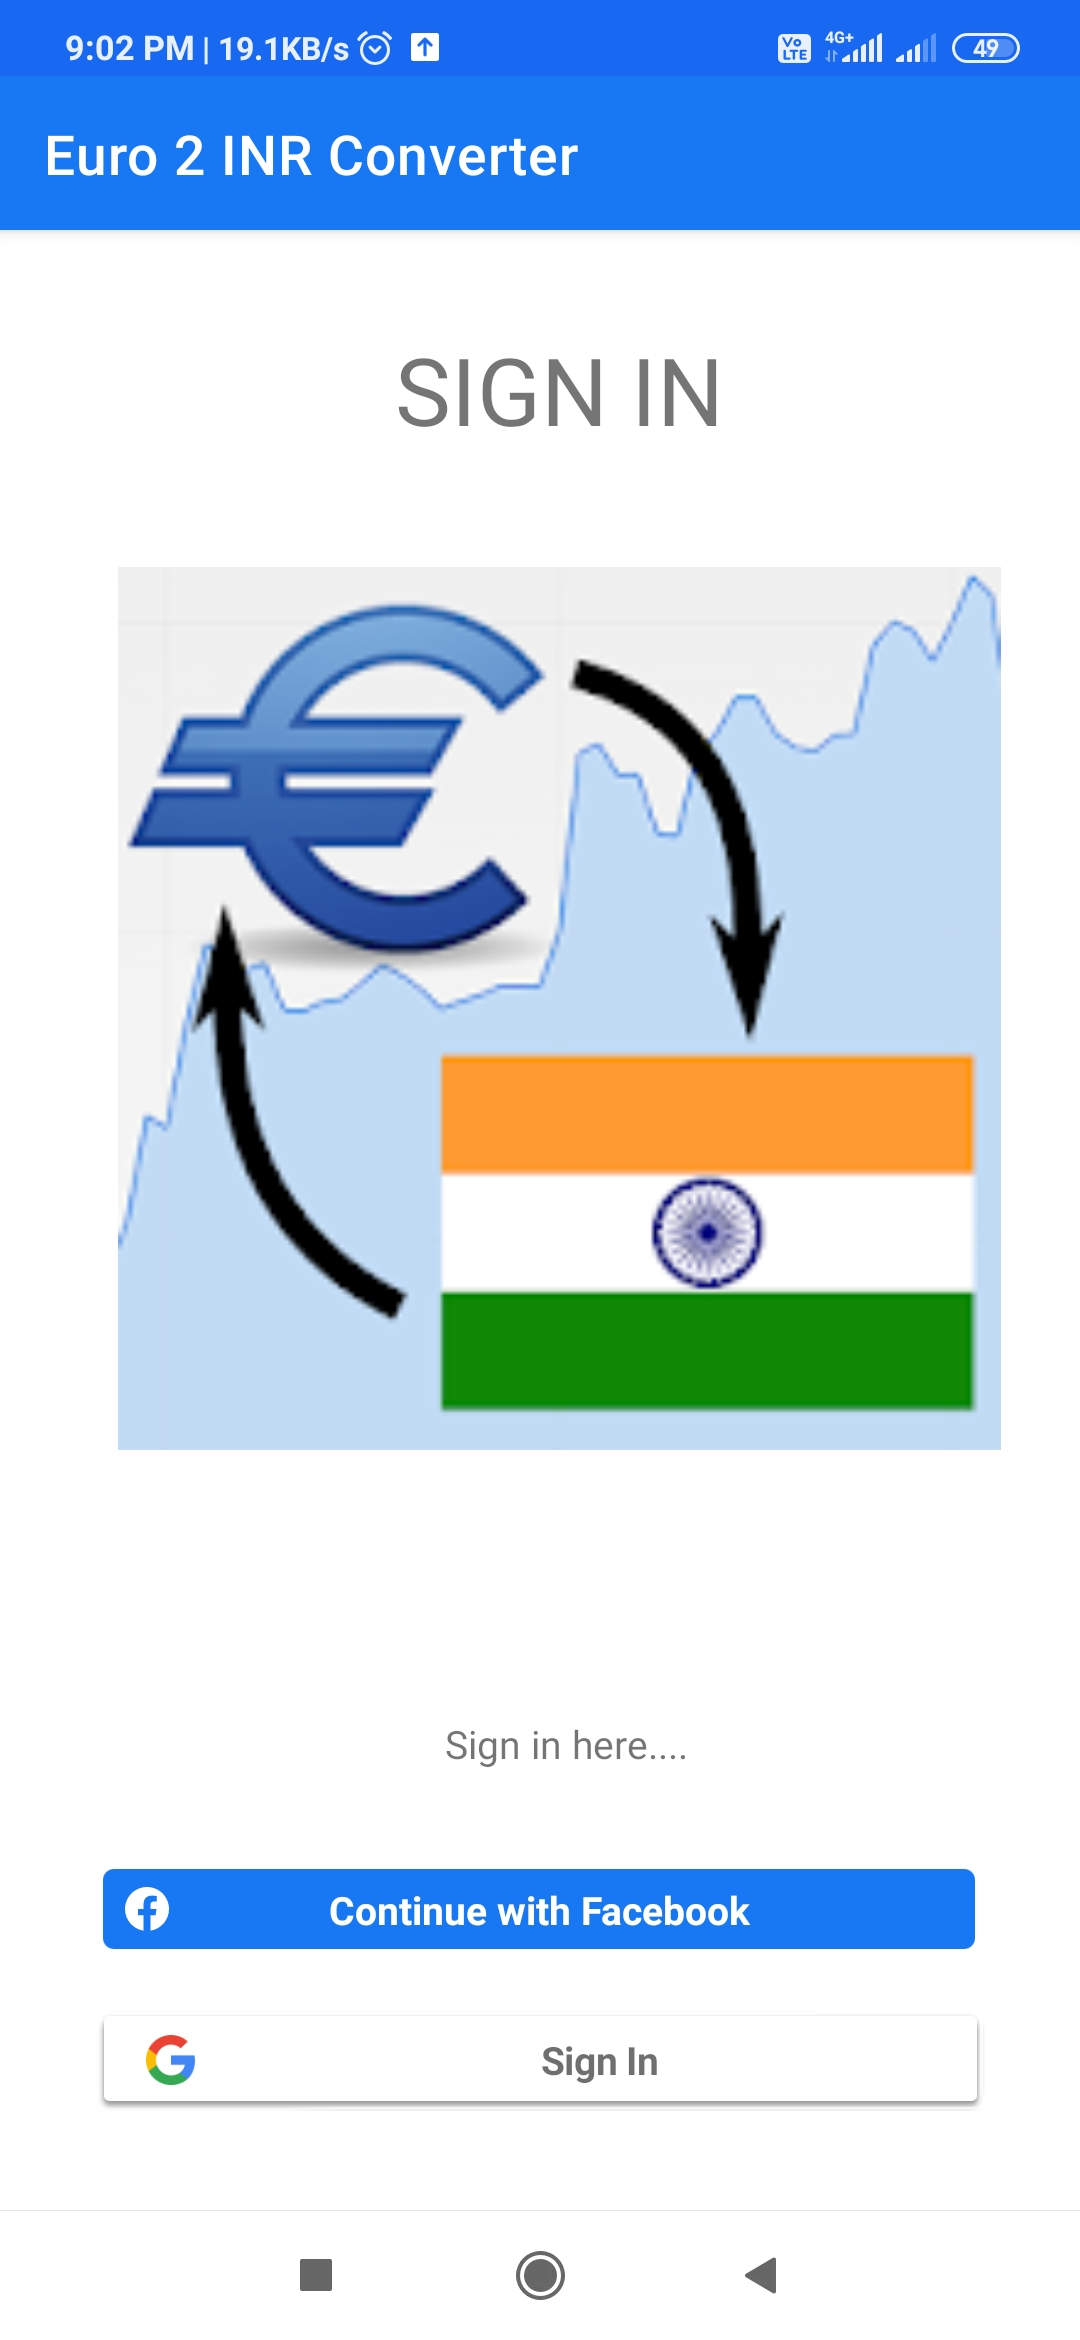
\includegraphics[scale=0.065]{146977676-a6f3eeb2-a4ef-4b31-bdde-234db3f75de1.jpg}
\caption{SignIn Page (i)}
\label{SignIn Page (i)}
\end{subfigure}
\hfill
\begin{subfigure}[h]{0.3\textwidth}
\centering
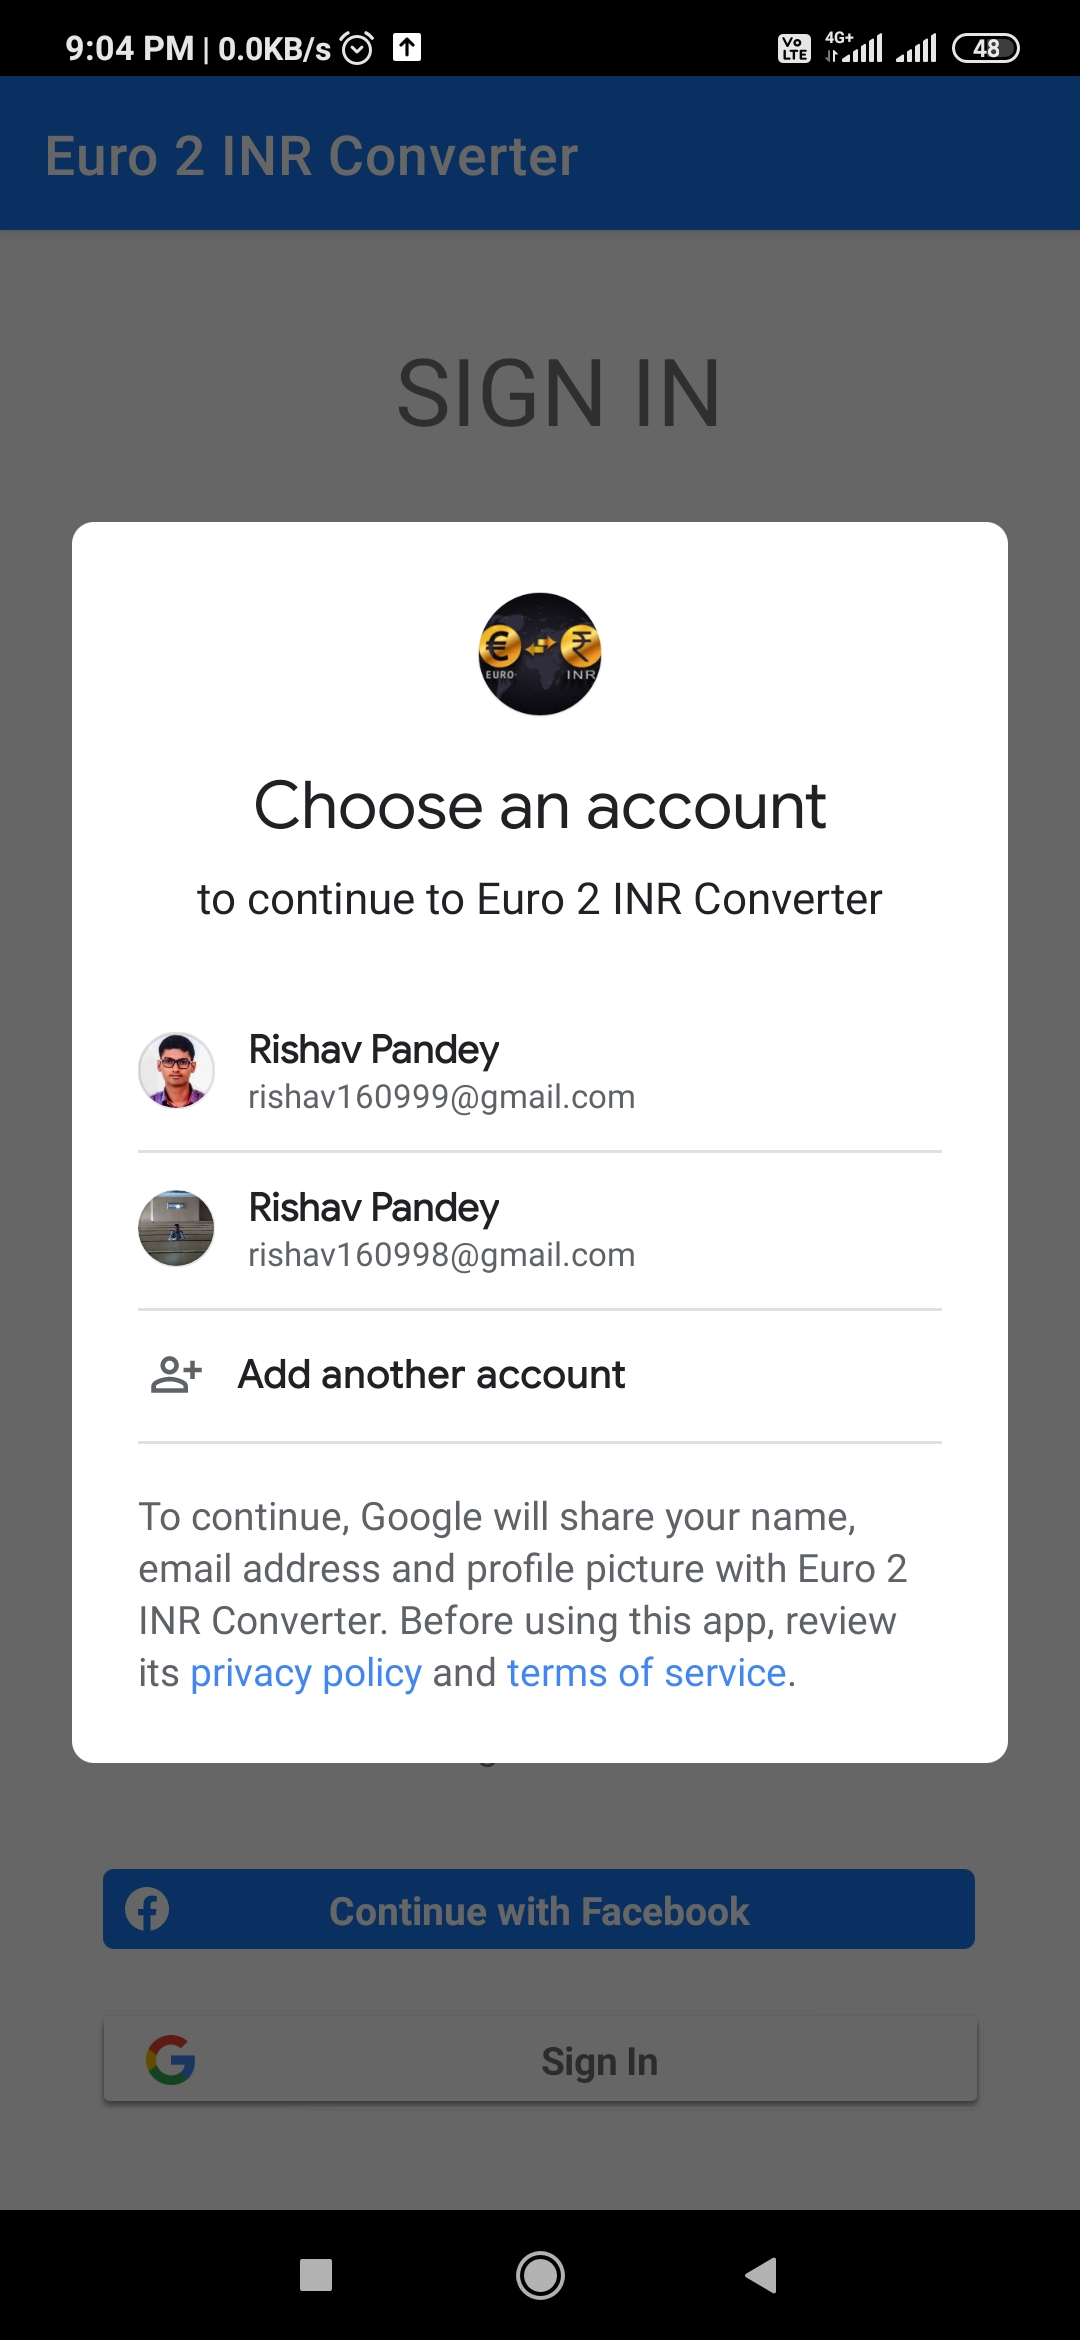
\includegraphics[scale=0.065]{146977794-37d93686-f927-4867-9725-8f424970e379.jpg}
\caption{SignIn Page (ii)}
\label{SignIn Page (ii)}
\end{subfigure}
\hfill
\begin{subfigure}[h]{0.3\textwidth}
\centering
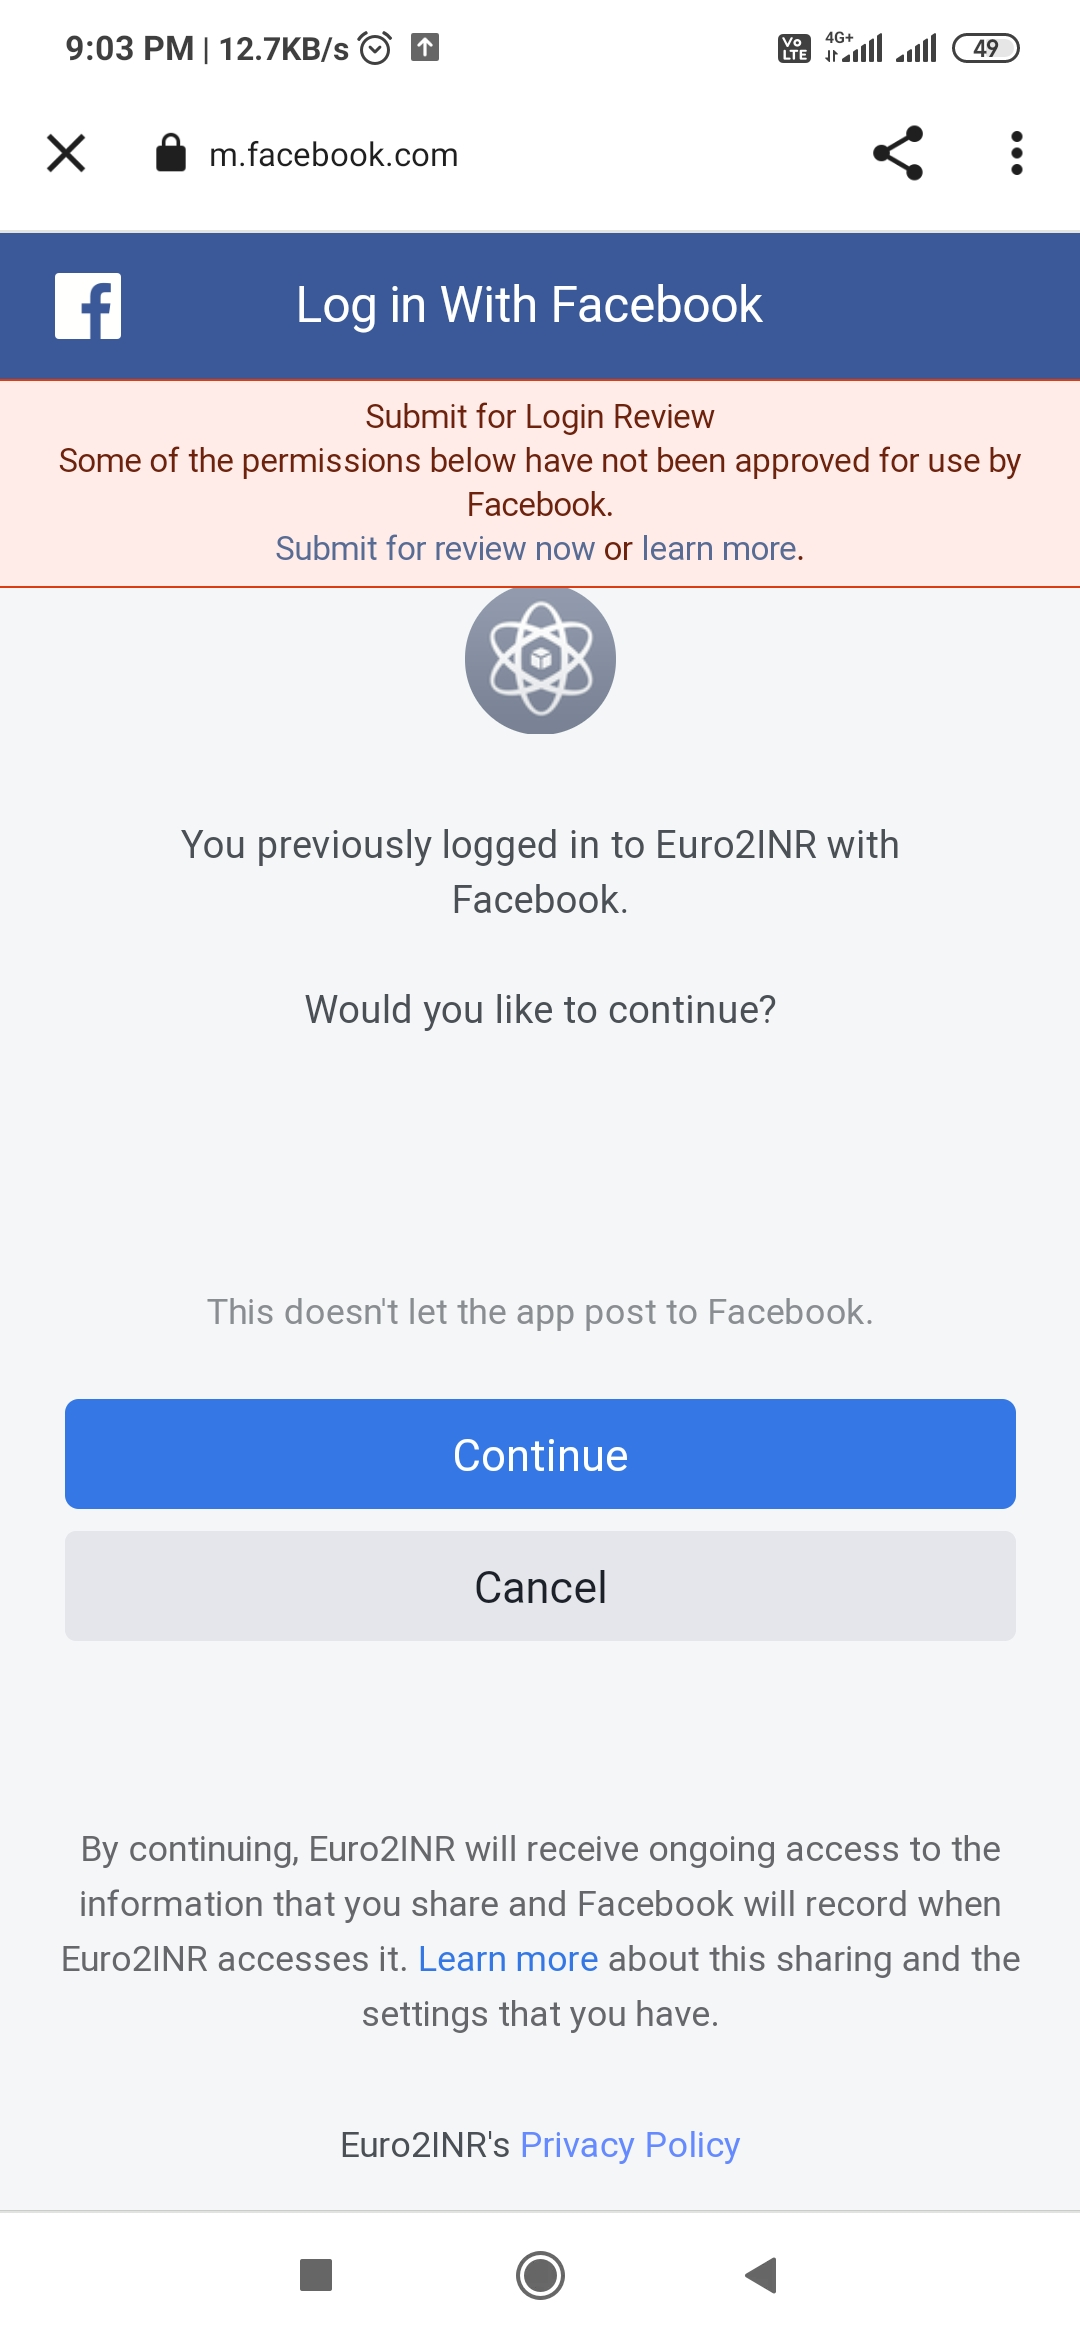
\includegraphics[scale=0.065]{146977733-f1145a34-ac72-4aaf-b907-f2fae2e42296.jpg}
\caption{SignIn Page (iii)}
\label{SignIn Page (iii)}
\end{subfigure}
\caption{SignIn Page}
\label{SignIn Page}
\end{figure}

\subsection{Profile Page:}

\begin{figure}[h]
\centering
\begin{subfigure}[h]{0.3\textwidth}
\centering
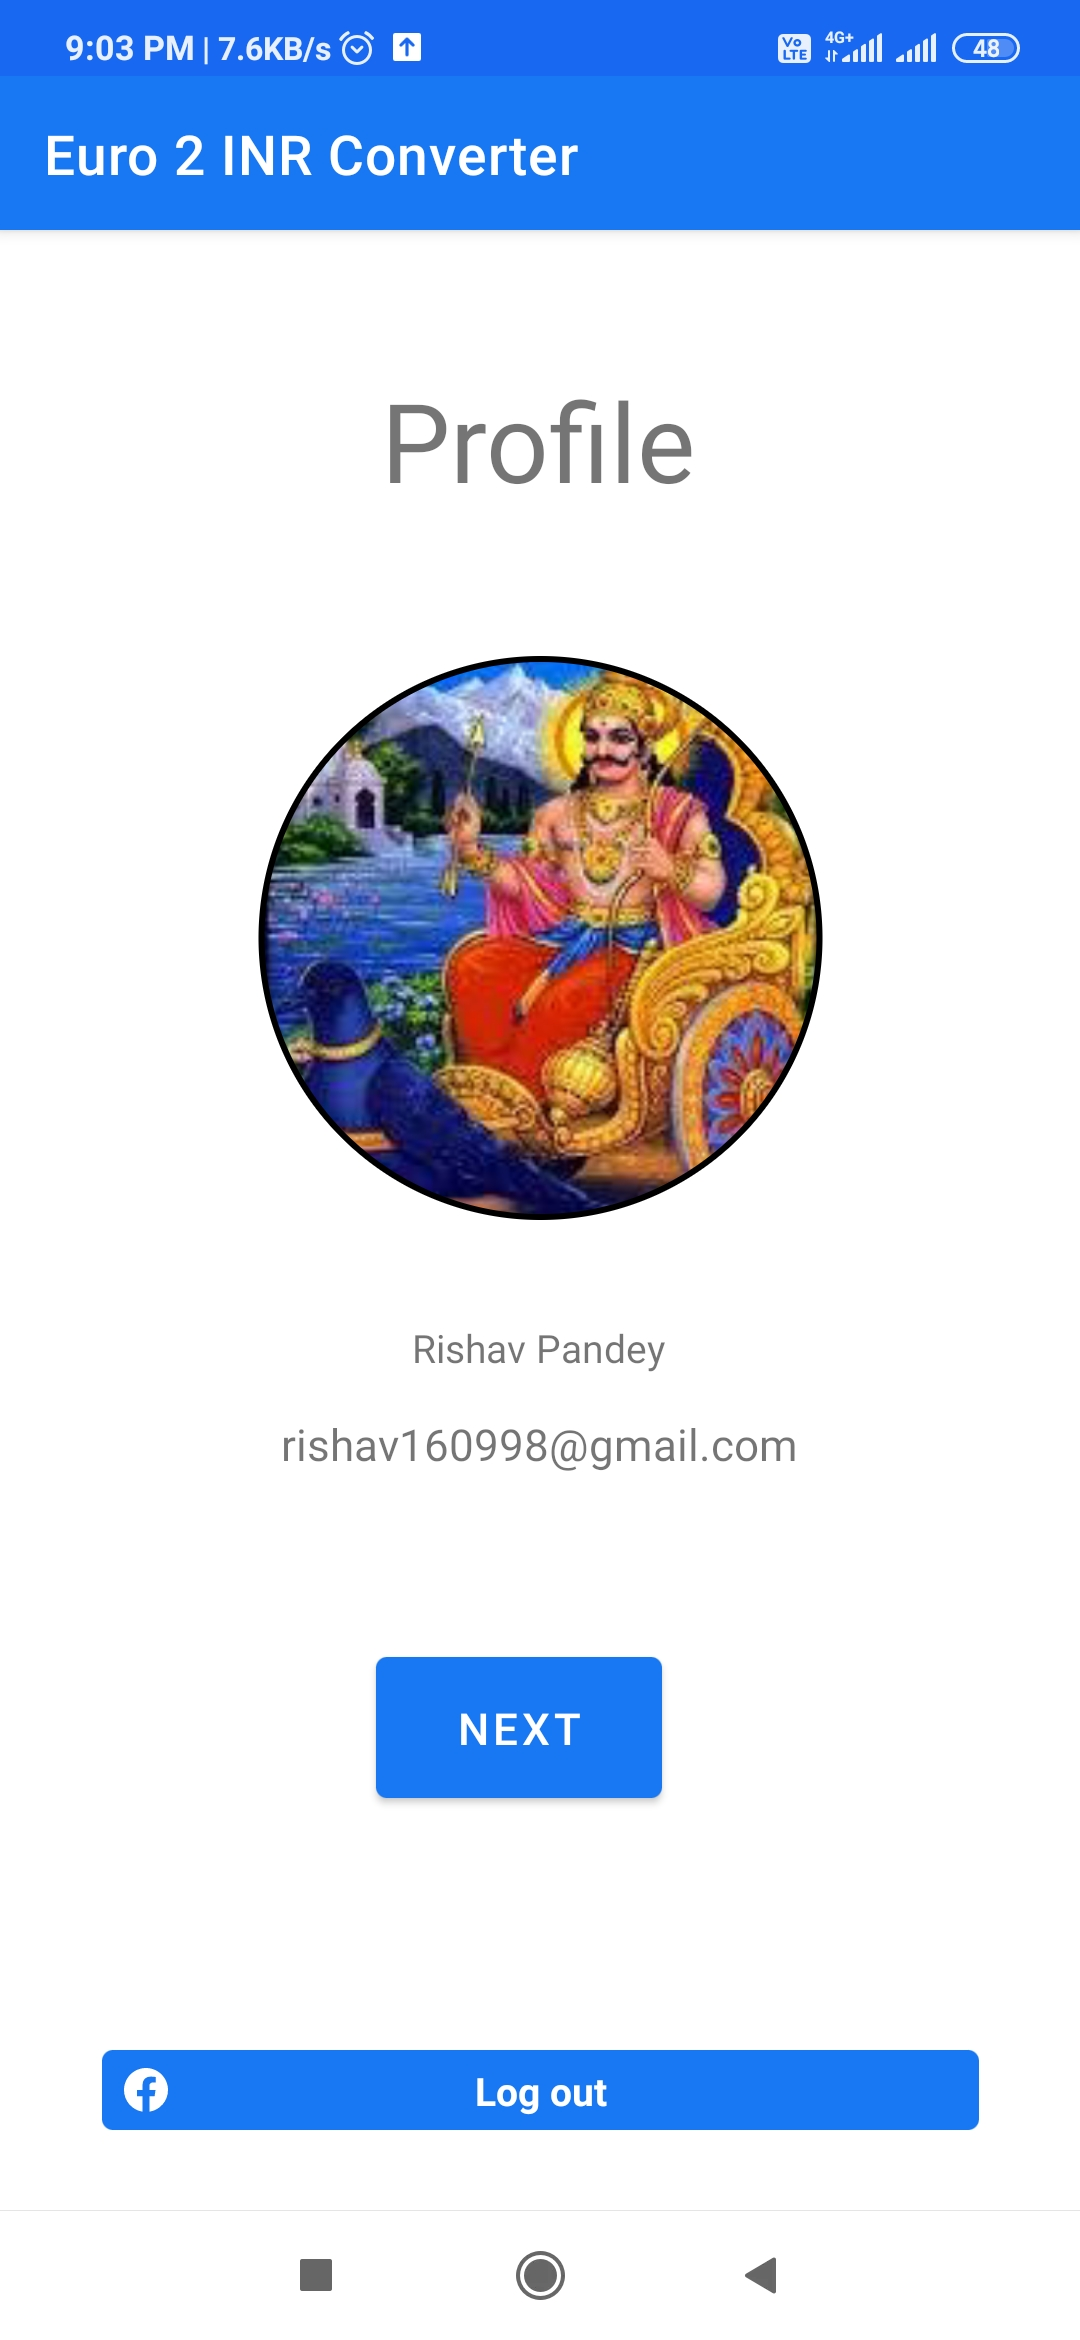
\includegraphics[scale=0.065]{146977758-1400c343-92b2-4aa8-b816-308310efb1fa.jpg}
\caption{Profile Page (i)}
\label{Profile Page (i)}
\end{subfigure}
\hfill
\begin{subfigure}[h]{0.3\textwidth}
\centering
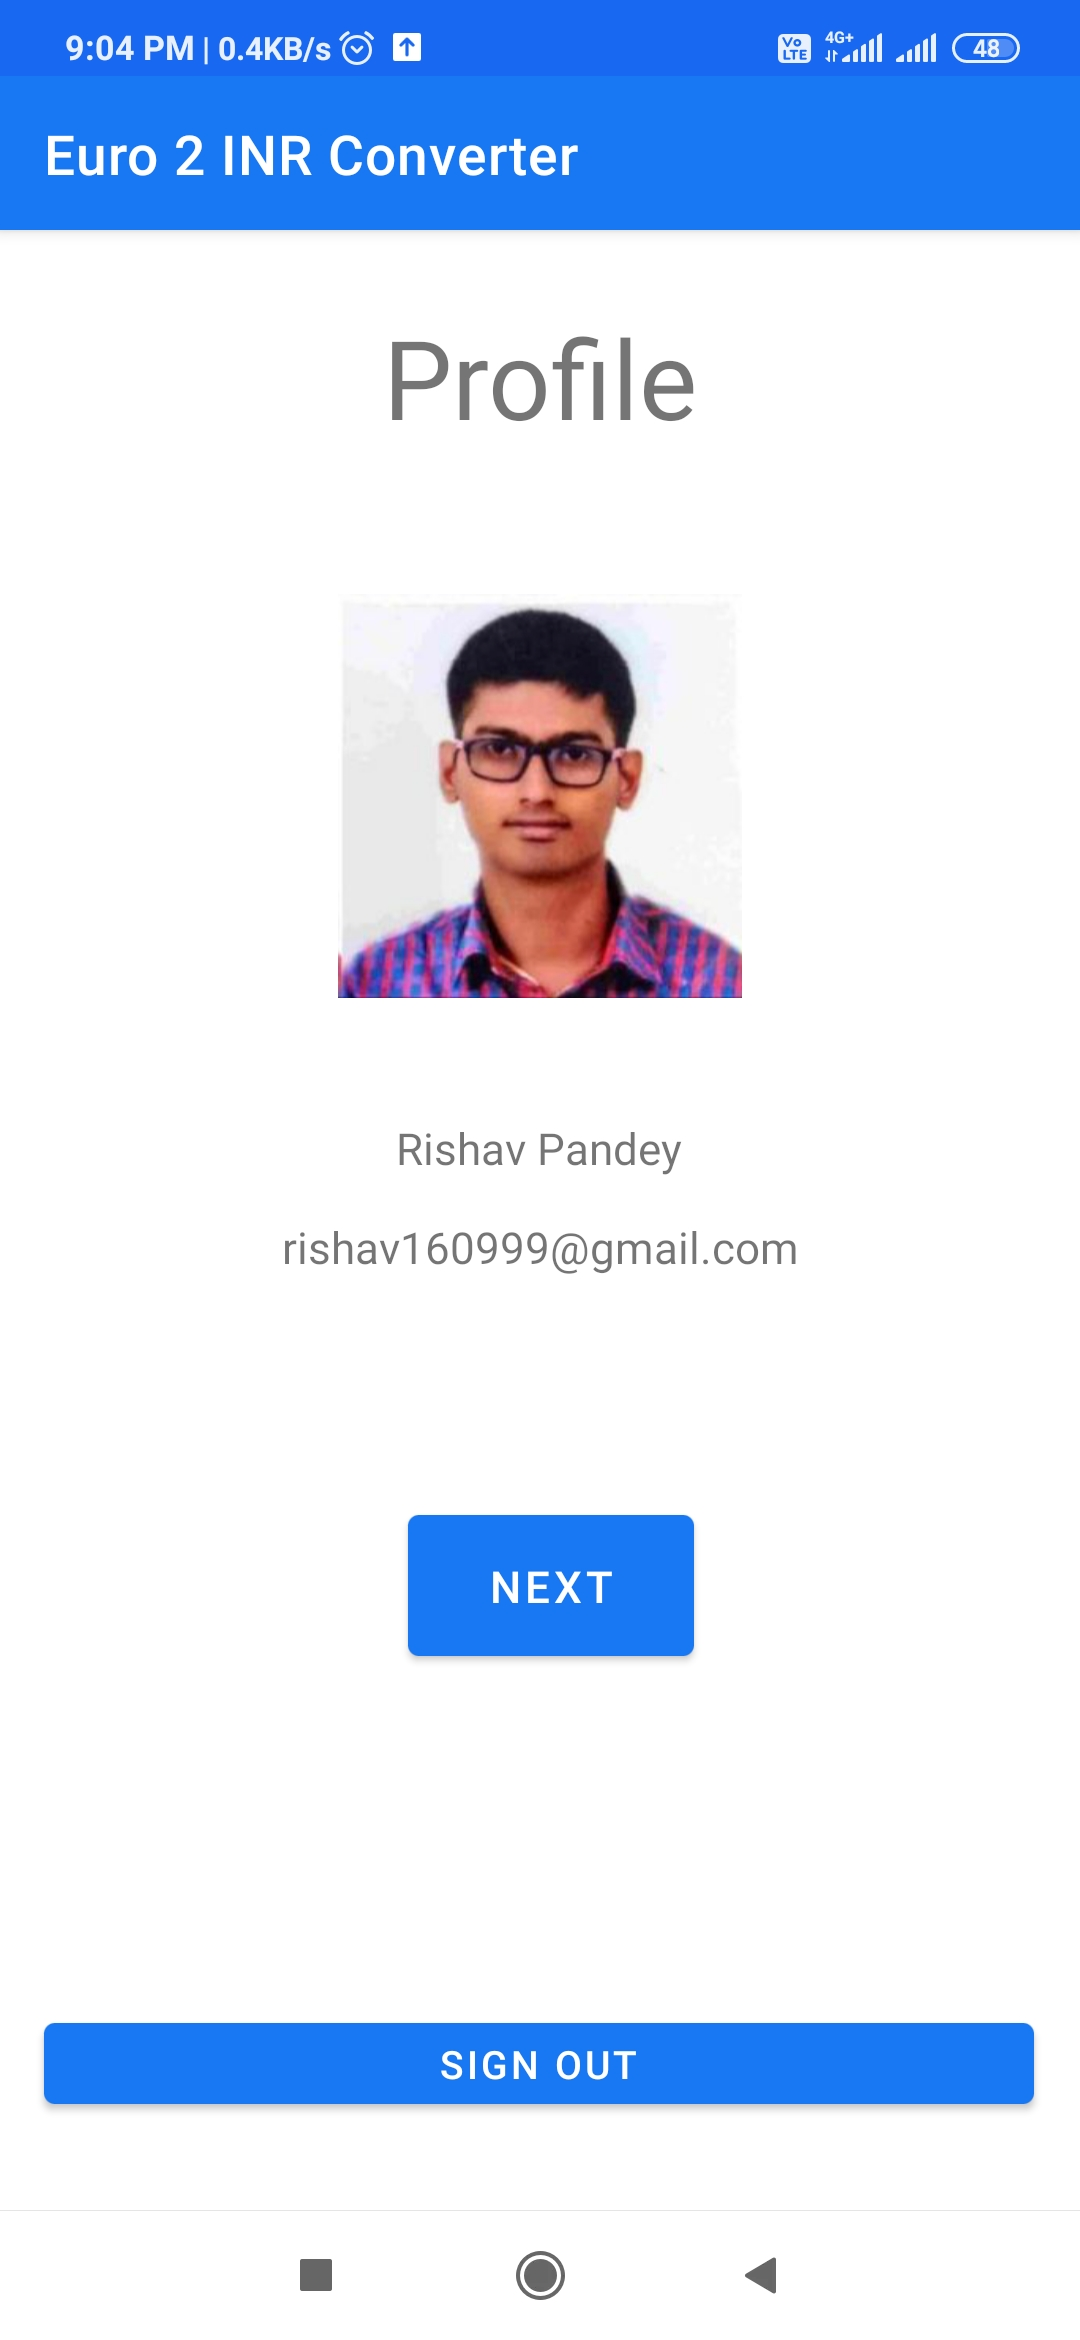
\includegraphics[scale=0.065]{146977809-c472db56-a7f6-495c-bf03-fbeea30632ab.jpg}
\caption{Profile Page (ii)}
\label{Profile Page (ii)}
\end{subfigure}
\hfill
\begin{subfigure}[h]{0.3\textwidth}
\centering
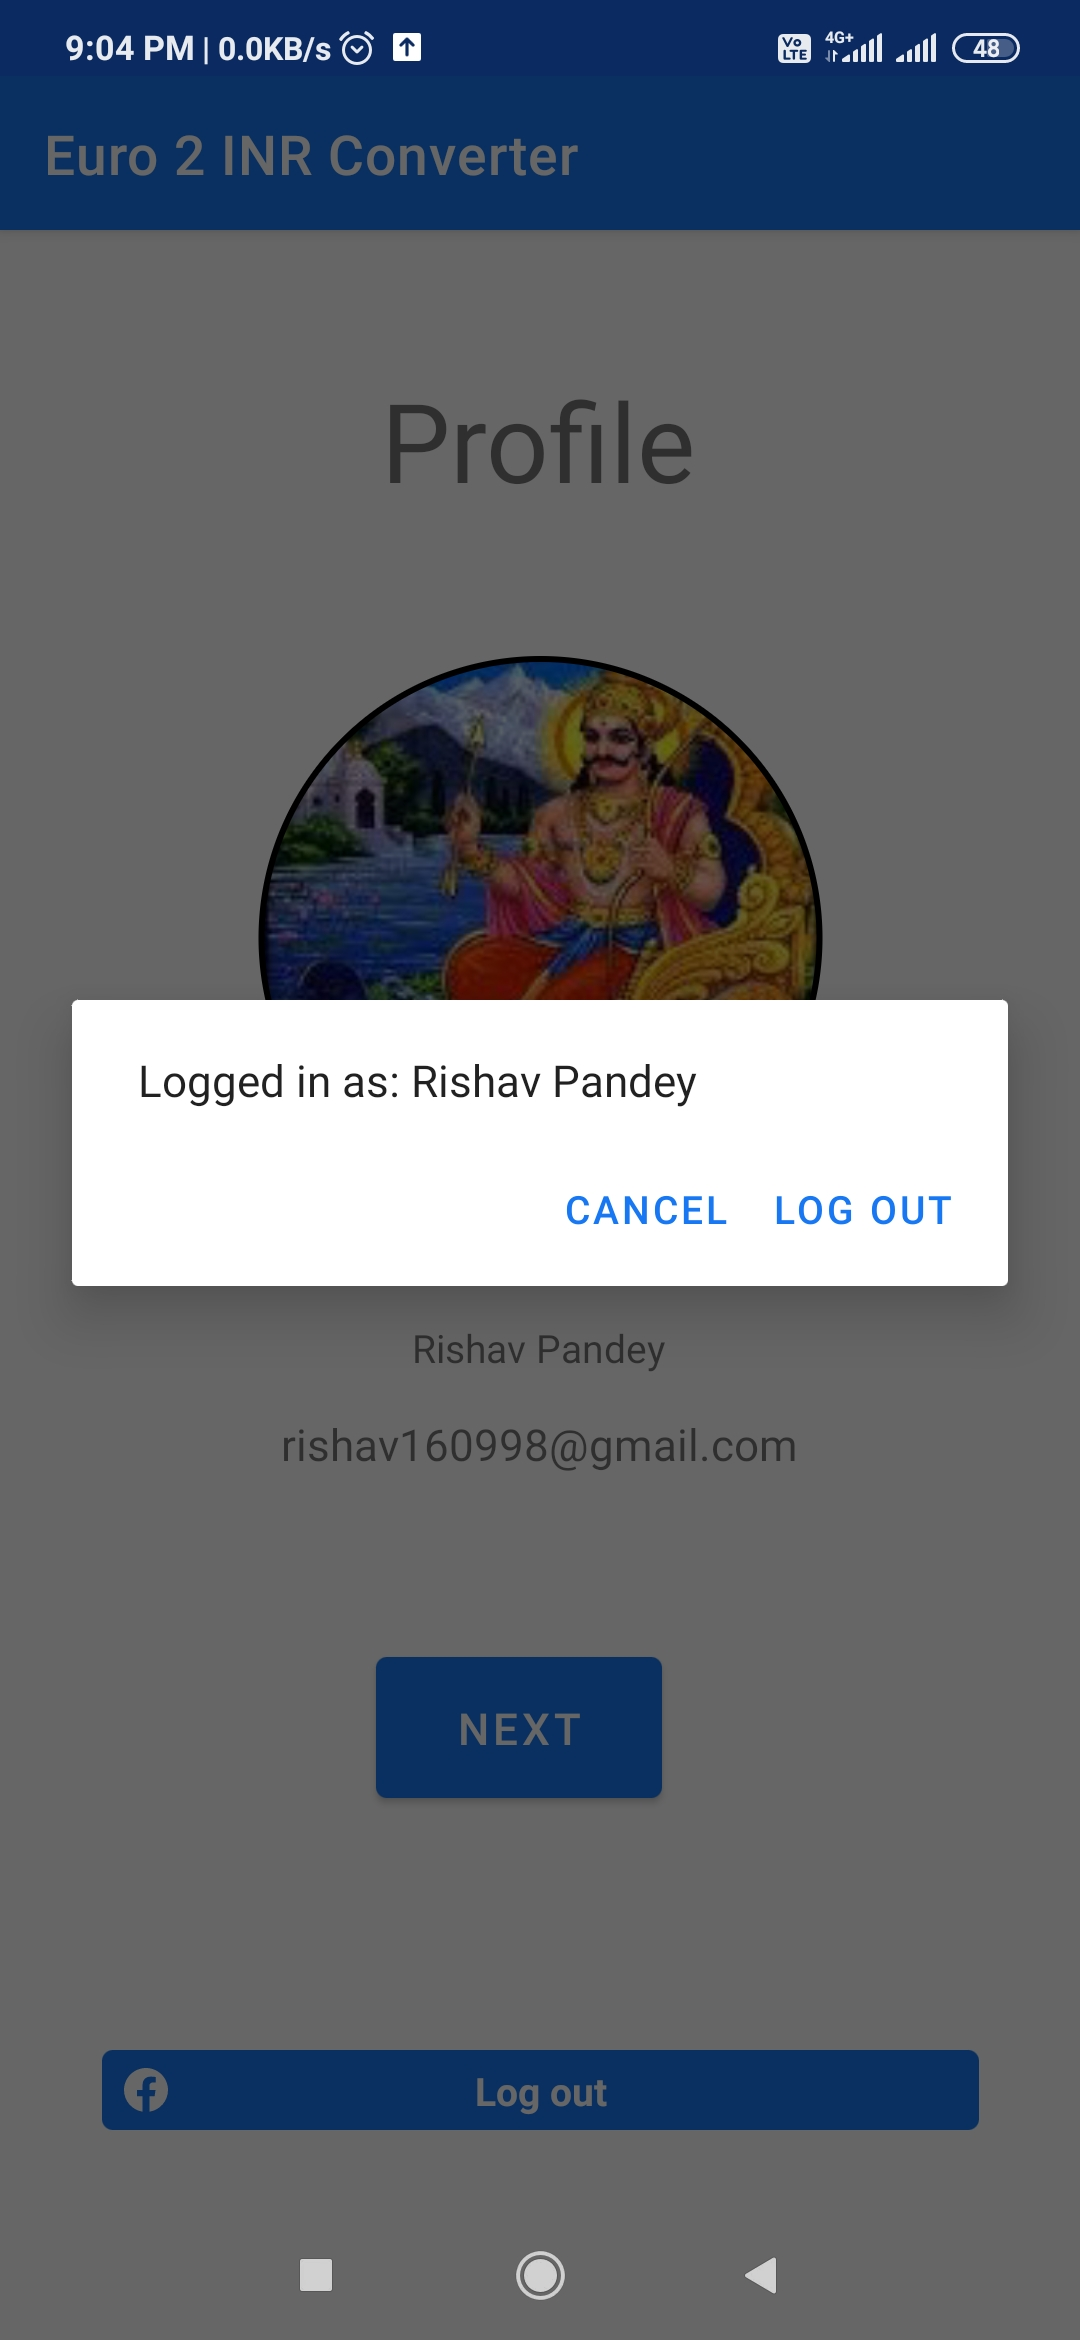
\includegraphics[scale=0.065]{146977781-d3ed2dc1-6e53-4d13-937d-9bafd6e2caa8.jpg}
\caption{Profile Page (iii)}
\label{Profile Page (iii)}
\end{subfigure}
\caption{Profile Page}
\label{Profile Page}
\end{figure}
\clearpage

\subsection{Euro-2-INR Convertor Page:}

\begin{figure}[h]
\centering
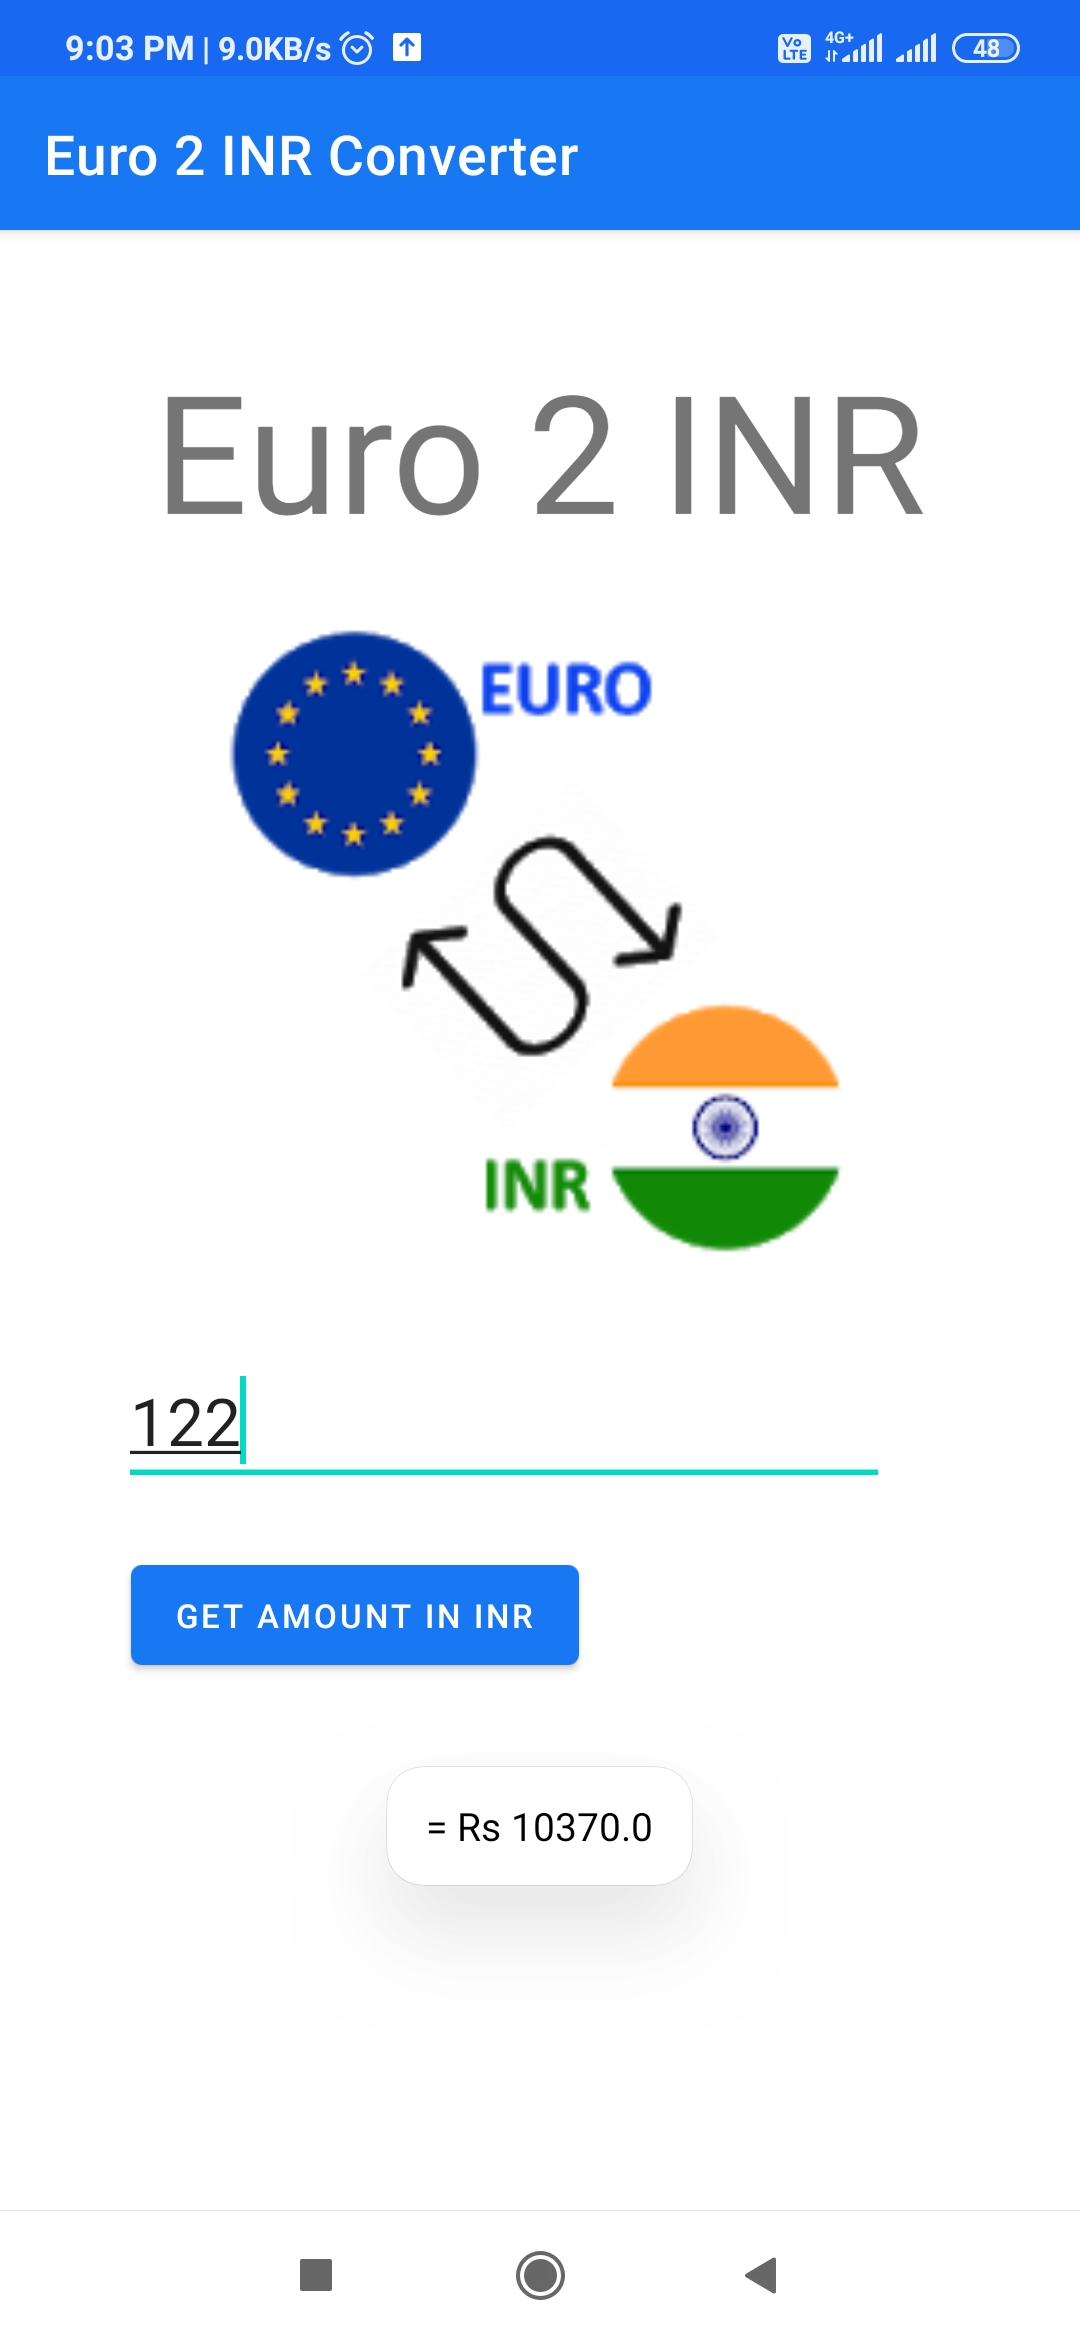
\includegraphics[scale=0.13]{146977771-f8aff4ba-14fa-4c17-8481-41be63a5799c.jpg}
\caption{Euro 2 INR Convertor Page}
\label{Euro 2 INR Convertor Page}
\end{figure}



\href{https://github.com/rishavpandey160999/Euro-2-INR-Converter}{GitHub Repo}\\

\href{https://youtu.be/AC3TEC7_Bi4}{Presentation}



\clearpage

\section{Works Carried Out In Task 3:}
Learnt about all the services offered by an extremely secure cloud service provider Amazon Web Services (AWS) and implemented practically by launching an AWS EC2 Instance. I even used other services of AWS like storage services (AWS S3) and security services (IAM).

After launching the instance, I secure shelled into the same and further hosted my portfolio website on that virtual server. [Figure \ref{Website live on AWS EC2}]

\subsection{Steps to host a website on AWS EC2 Instance:}\cite{mishra2017amazon}\\
\\
\textbf{Step 1:} Choose an Amazon Machine Image (AMI).
\begin{figure}[h]
\centering
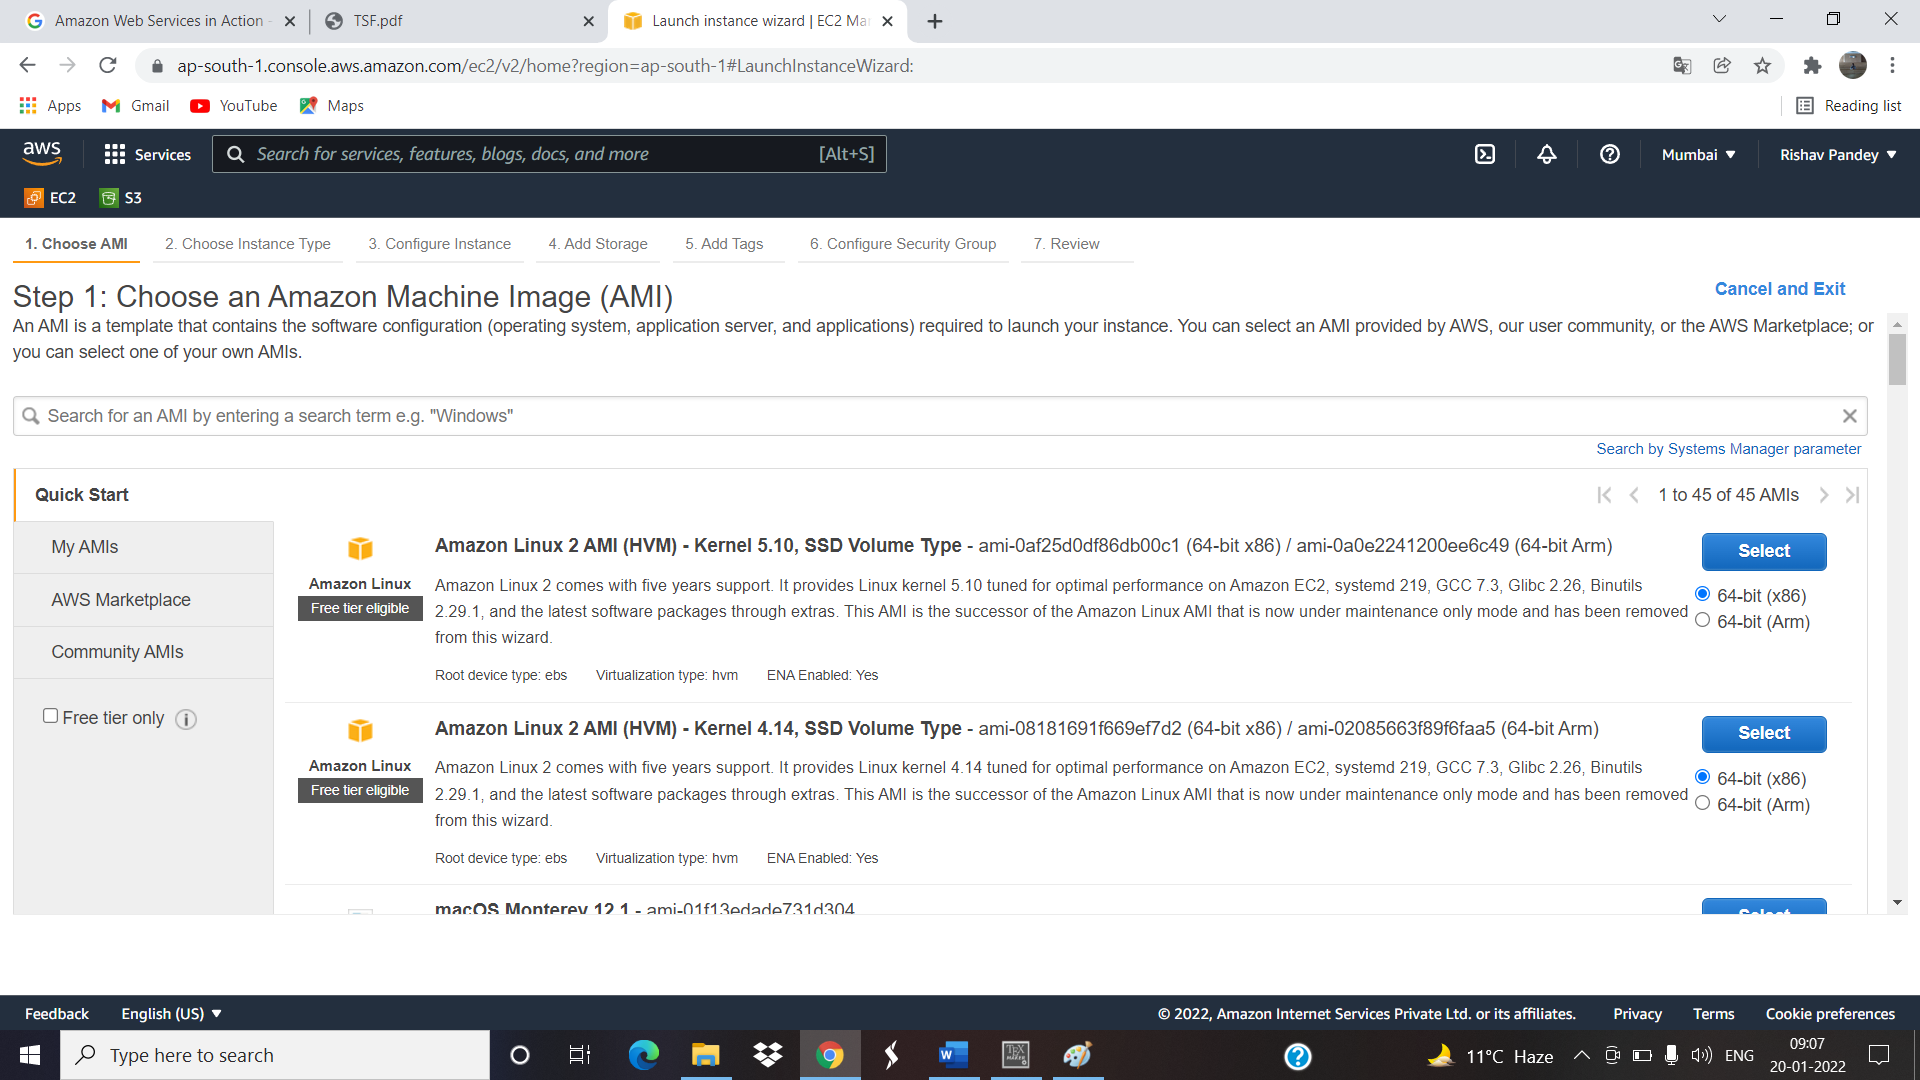
\includegraphics[scale=0.3]{Untitled6.png}
\caption{Choose an Amazon Machine Image}
\label{Choose an Amazon Machine Image}
\end{figure}
\clearpage

\textbf{Step 2:} Choose an Instance Type.
\begin{figure}[h]
\centering
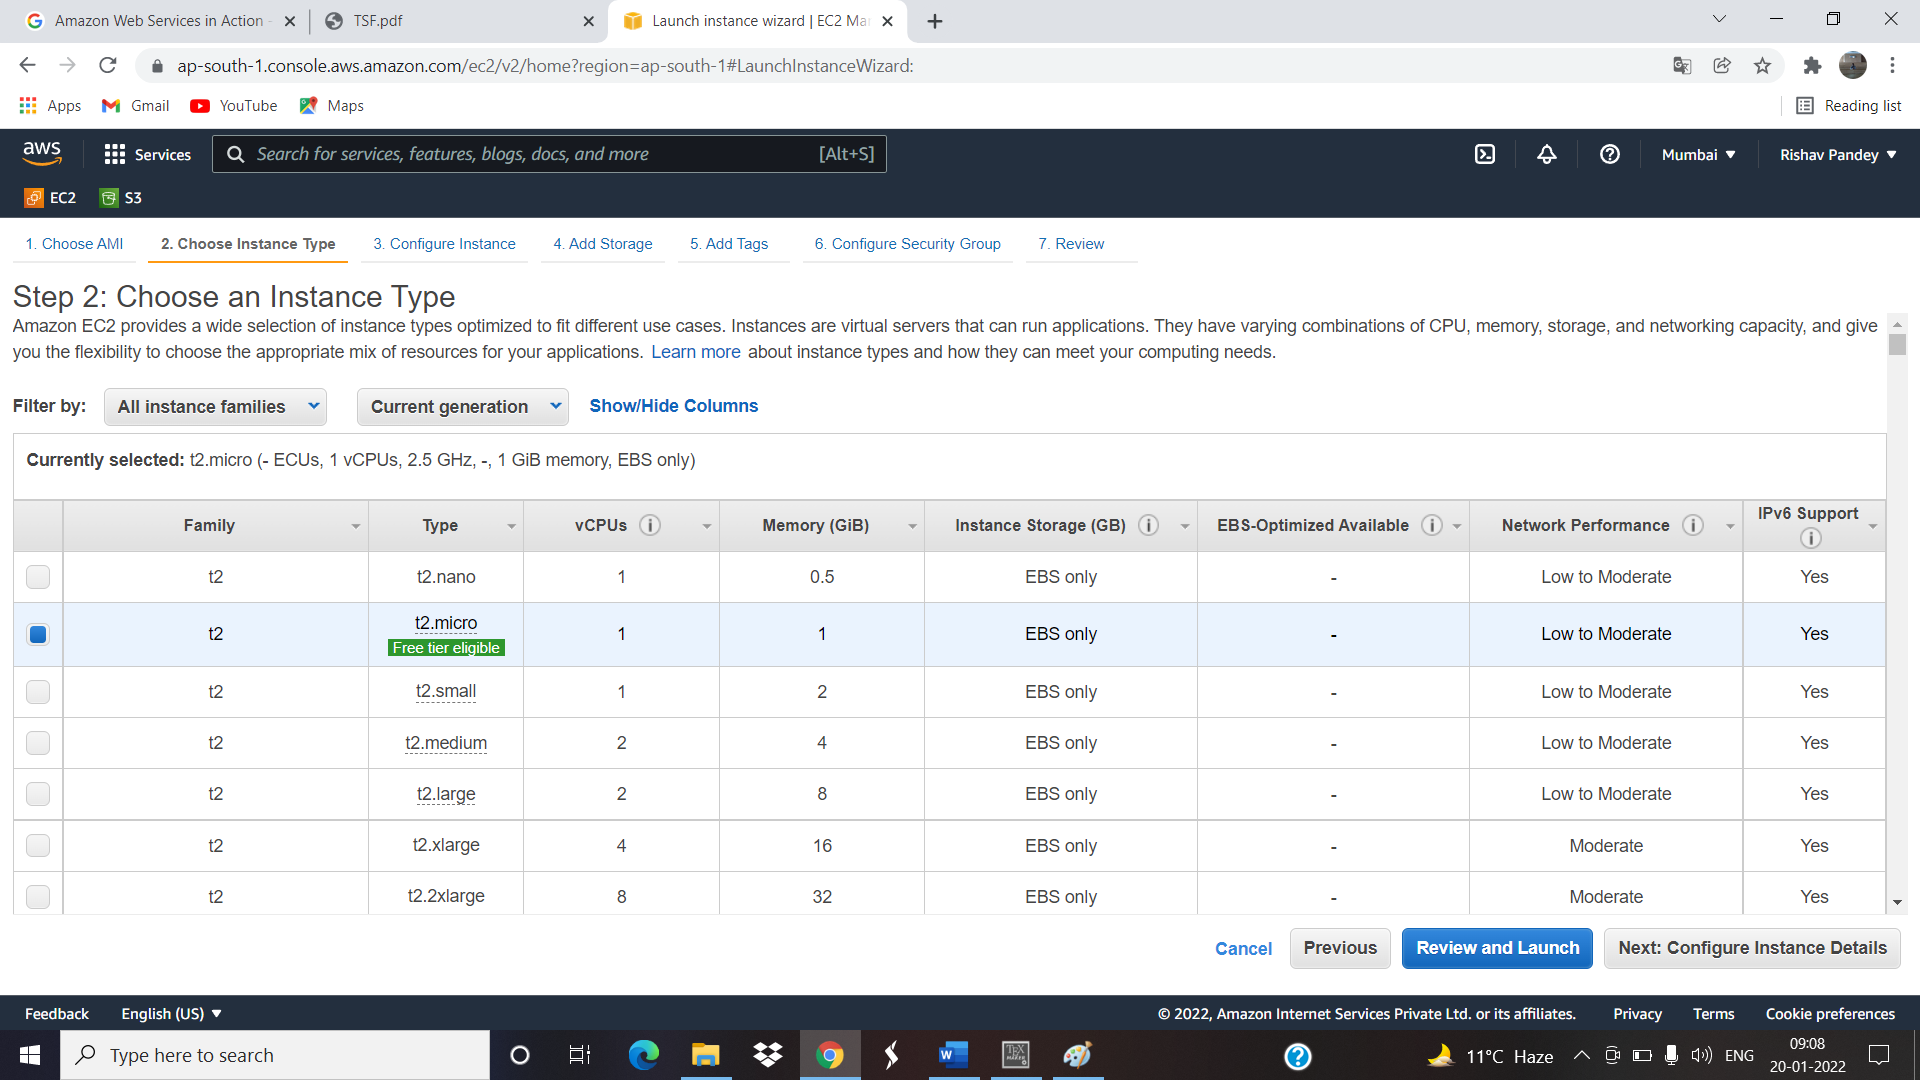
\includegraphics[scale=0.265]{Untitled7.png}
\caption{Choose an Instance Type}
\label{Choose an Instance Type}
\end{figure}

\textbf{Step 3:} Configure Instance Details.
\begin{figure}[h]
\centering
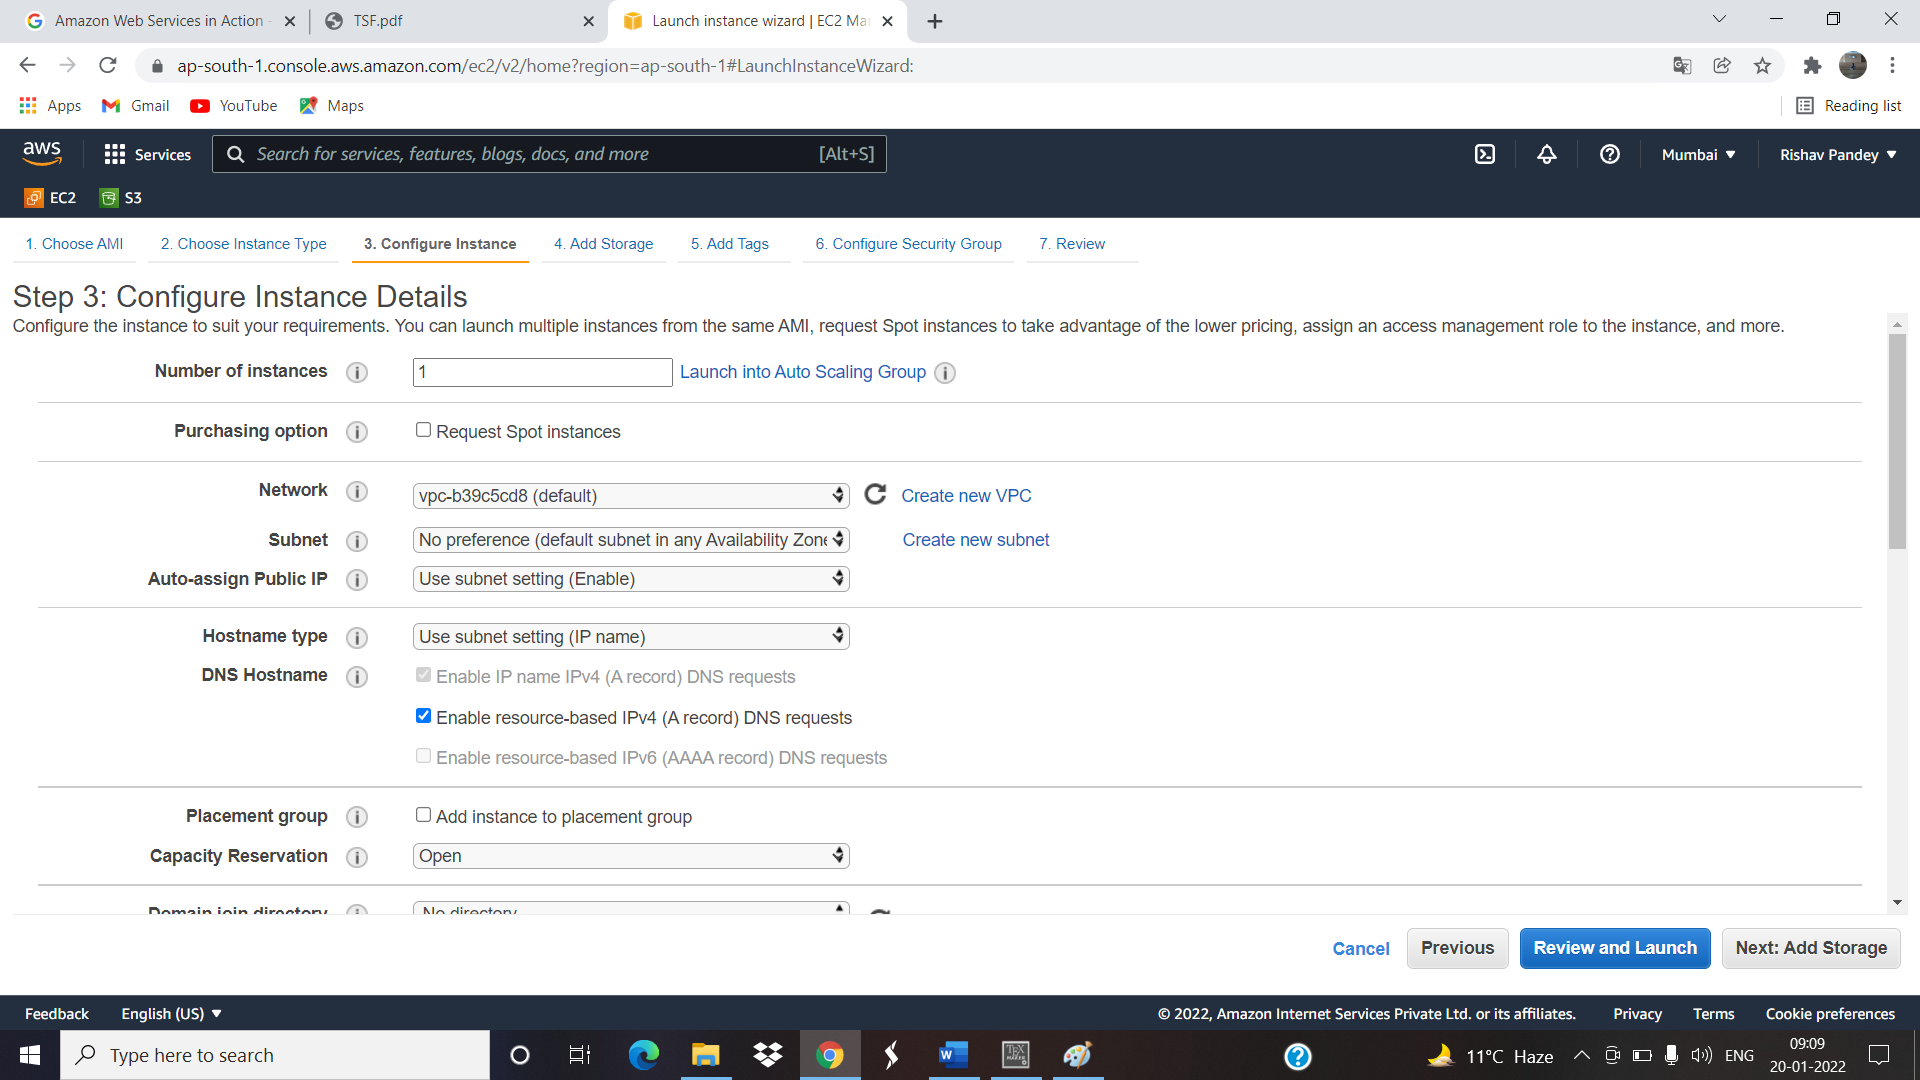
\includegraphics[scale=0.265]{Untitled8.png}
\caption{Configure Instance Details}
\label{Configure Instance Details}
\end{figure}
\clearpage

\textbf{Step 4:} Add Storage.
\begin{figure}[h]
\centering
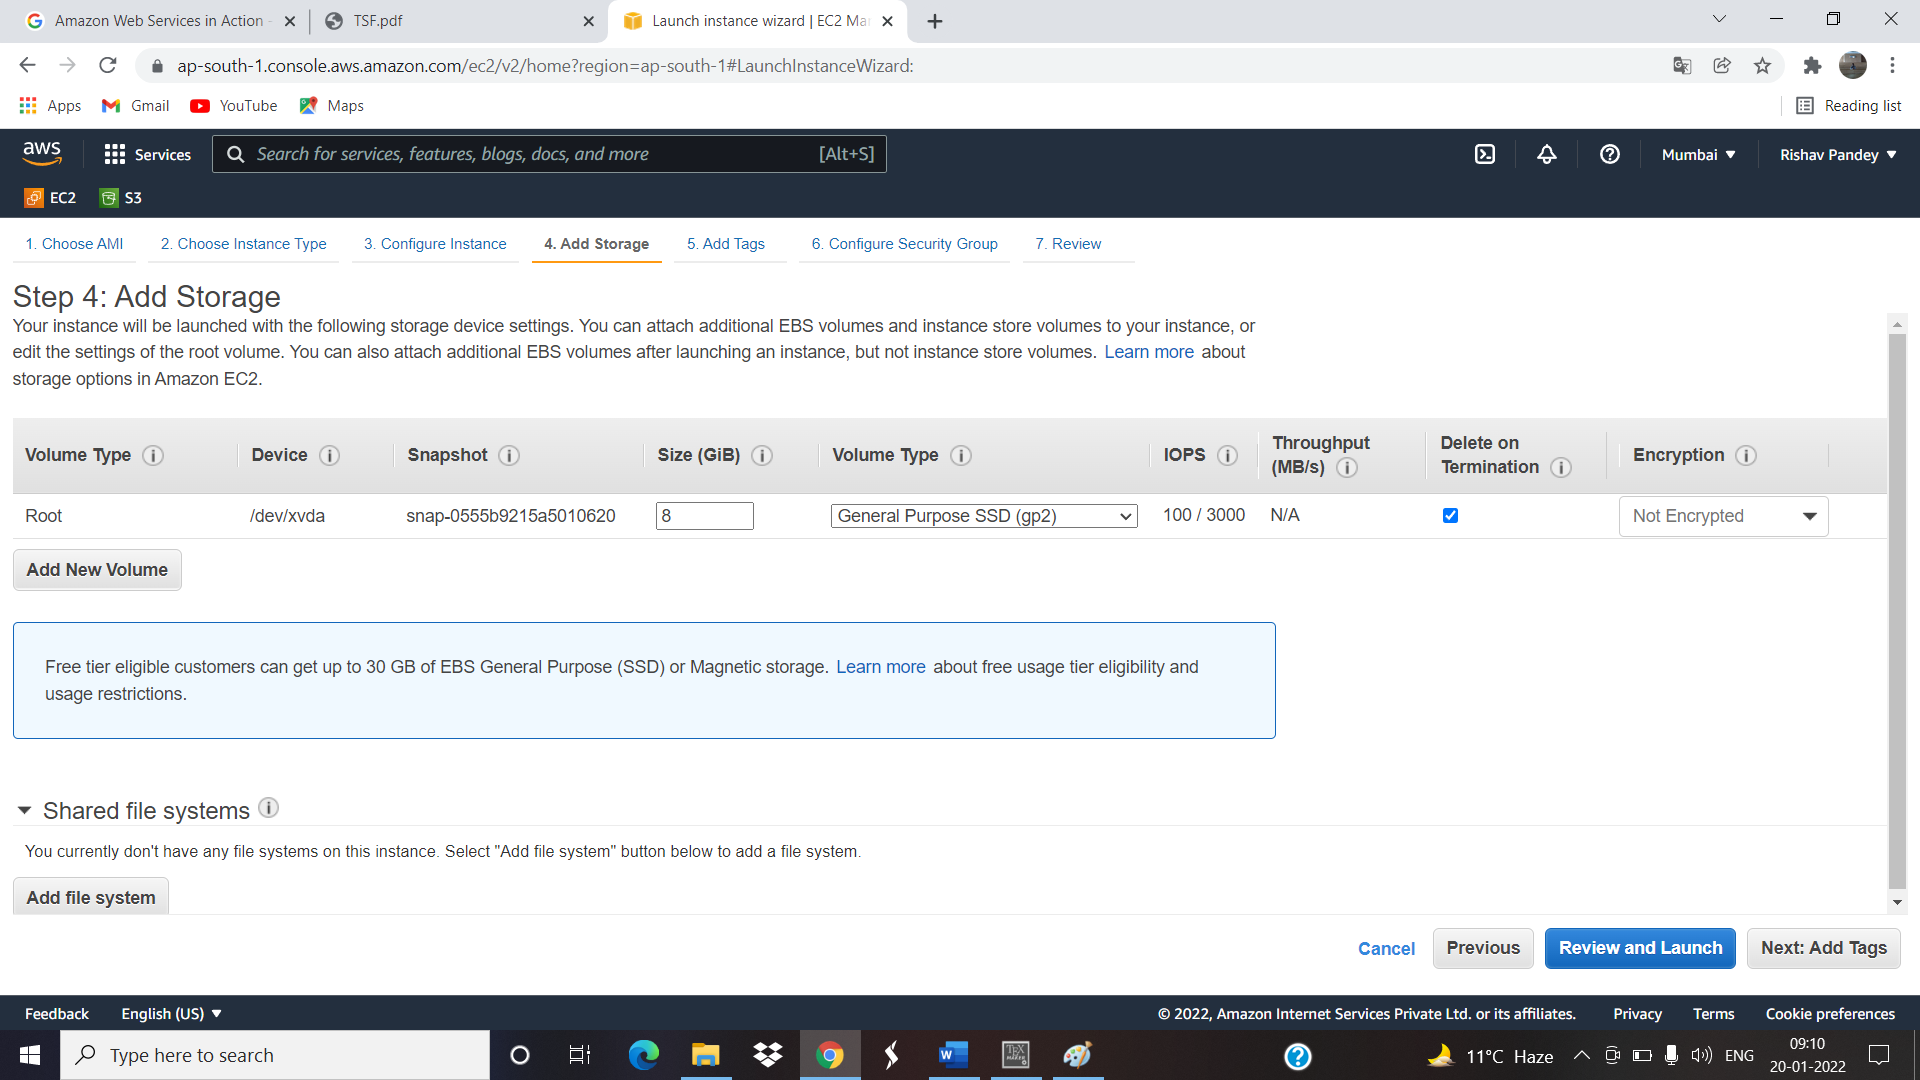
\includegraphics[scale=0.265]{Untitled9.png}
\caption{Add Storage}
\label{Add Storage}
\end{figure}

\textbf{Step 5:} Add Tags.
\begin{figure}[h]
\centering
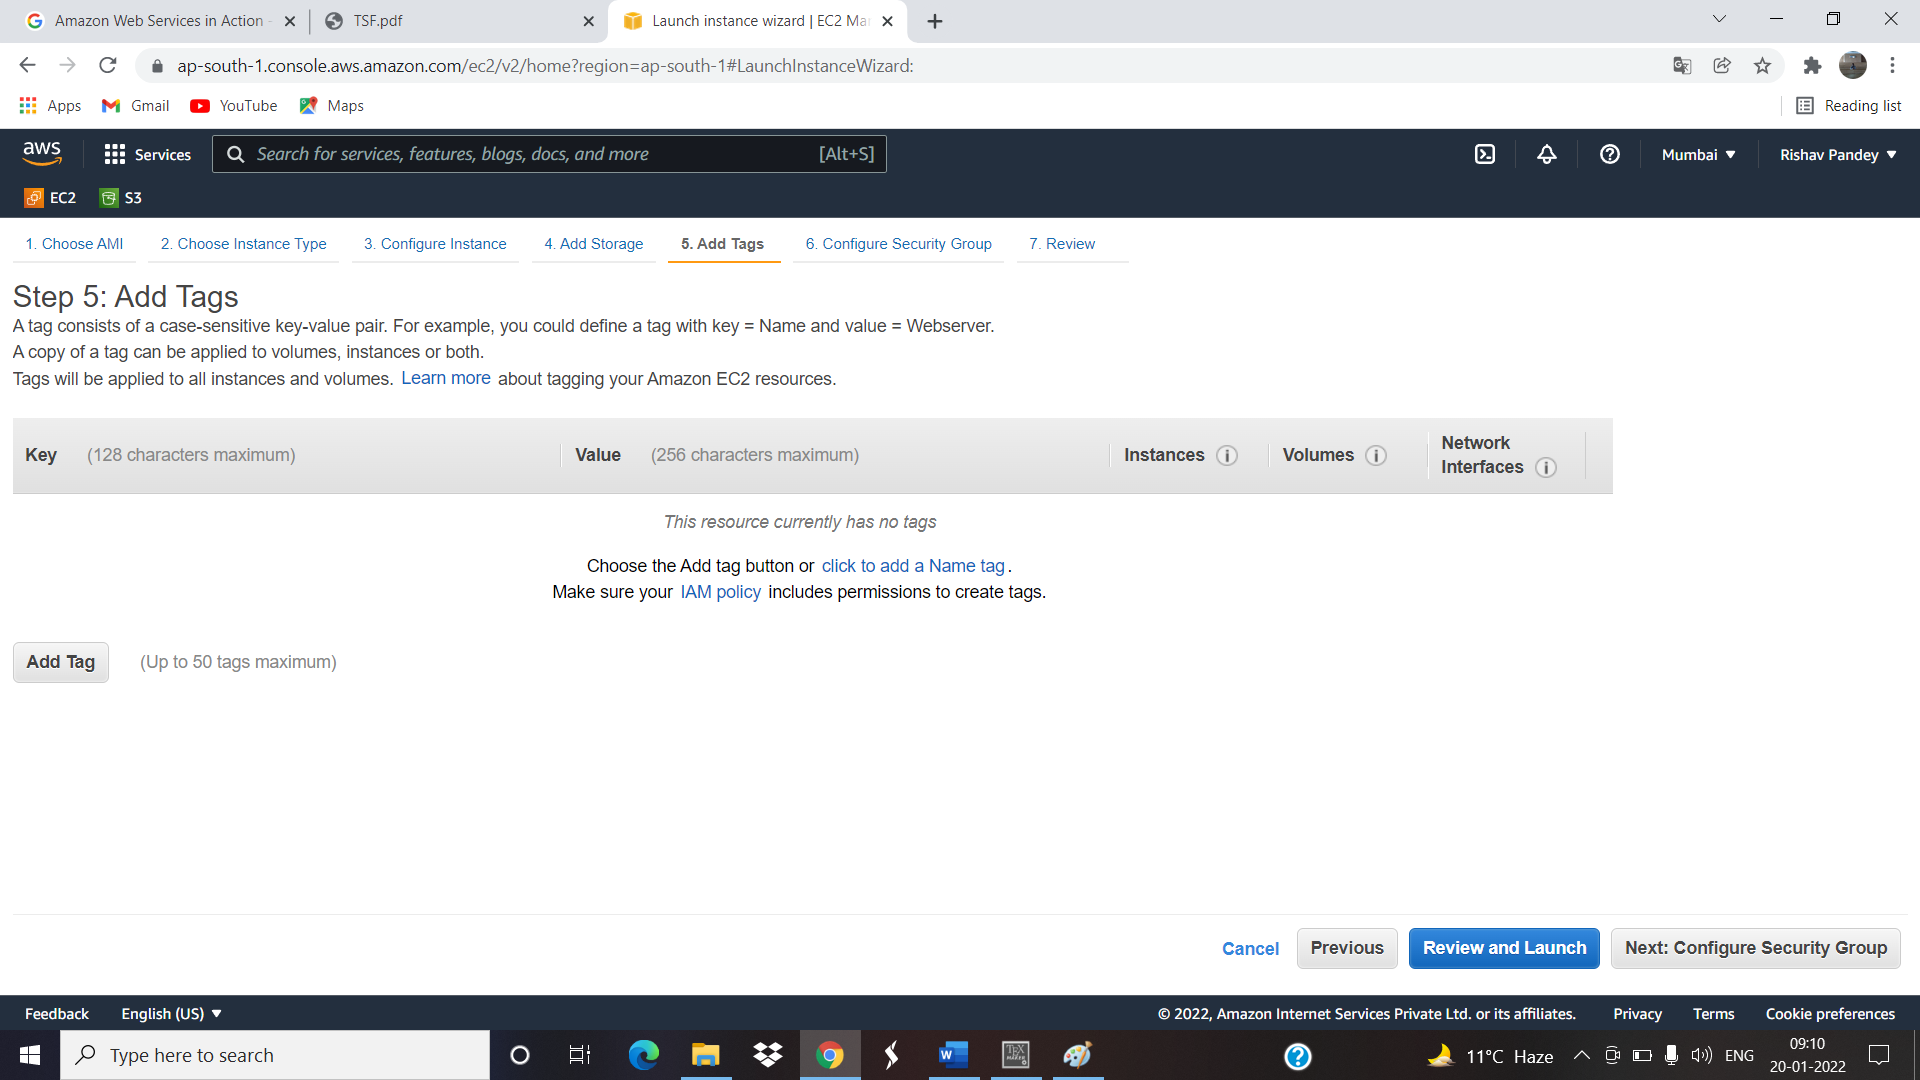
\includegraphics[scale=0.265]{Untitled10.png}
\caption{Add Tags}
\label{Add Tags}
\end{figure}
\clearpage

\textbf{Step 6:} Configure Security Group.
\begin{figure}[h]
\centering
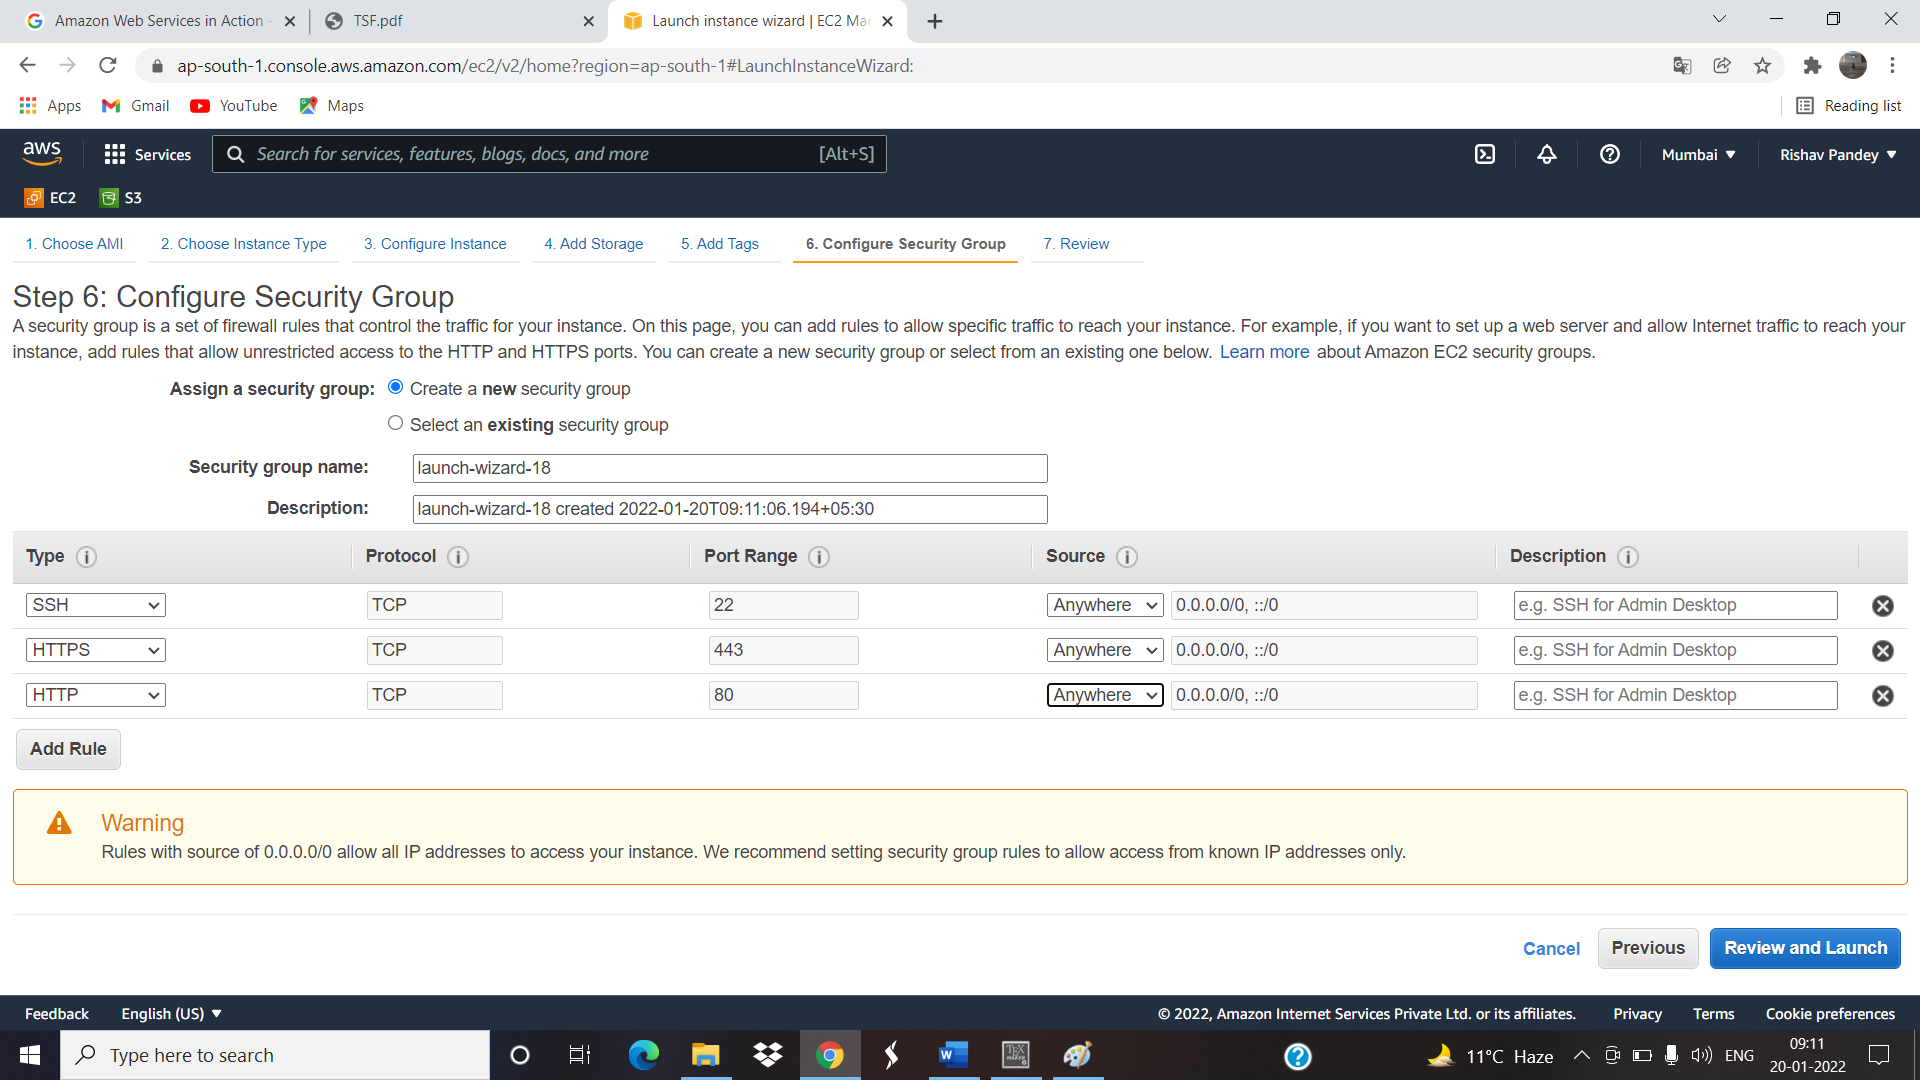
\includegraphics[scale=0.265]{Untitled11.png}
\caption{Configure Security Group}
\label{Configure Security Group}
\end{figure}

\textbf{Step 7:} Review Instance Launch.
\begin{figure}[h]
\centering
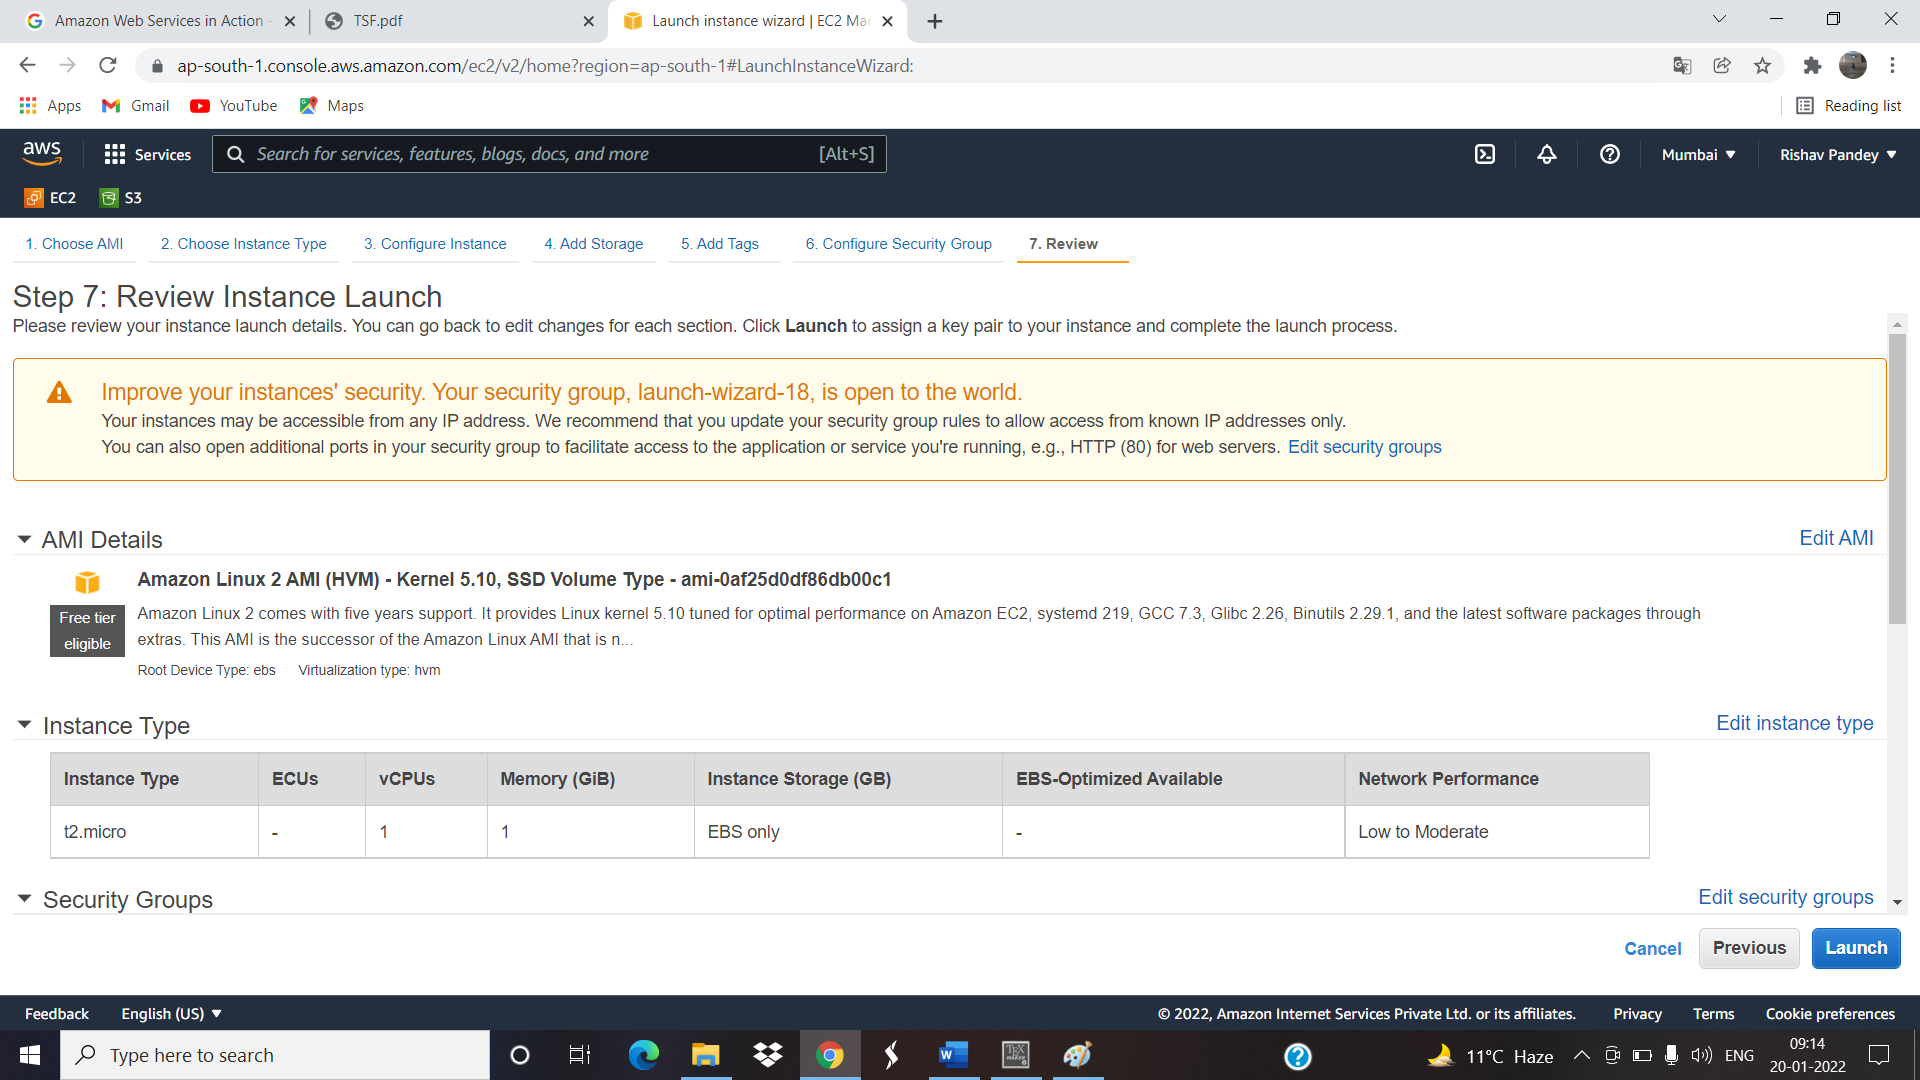
\includegraphics[scale=0.265]{Untitled12.png}
\caption{Review Instance Launch}
\label{Review Instance Launch}
\end{figure}
\clearpage

\textbf{Step 8:} Select an existing keypair or create a new key pair.
\begin{figure}[h]
\centering
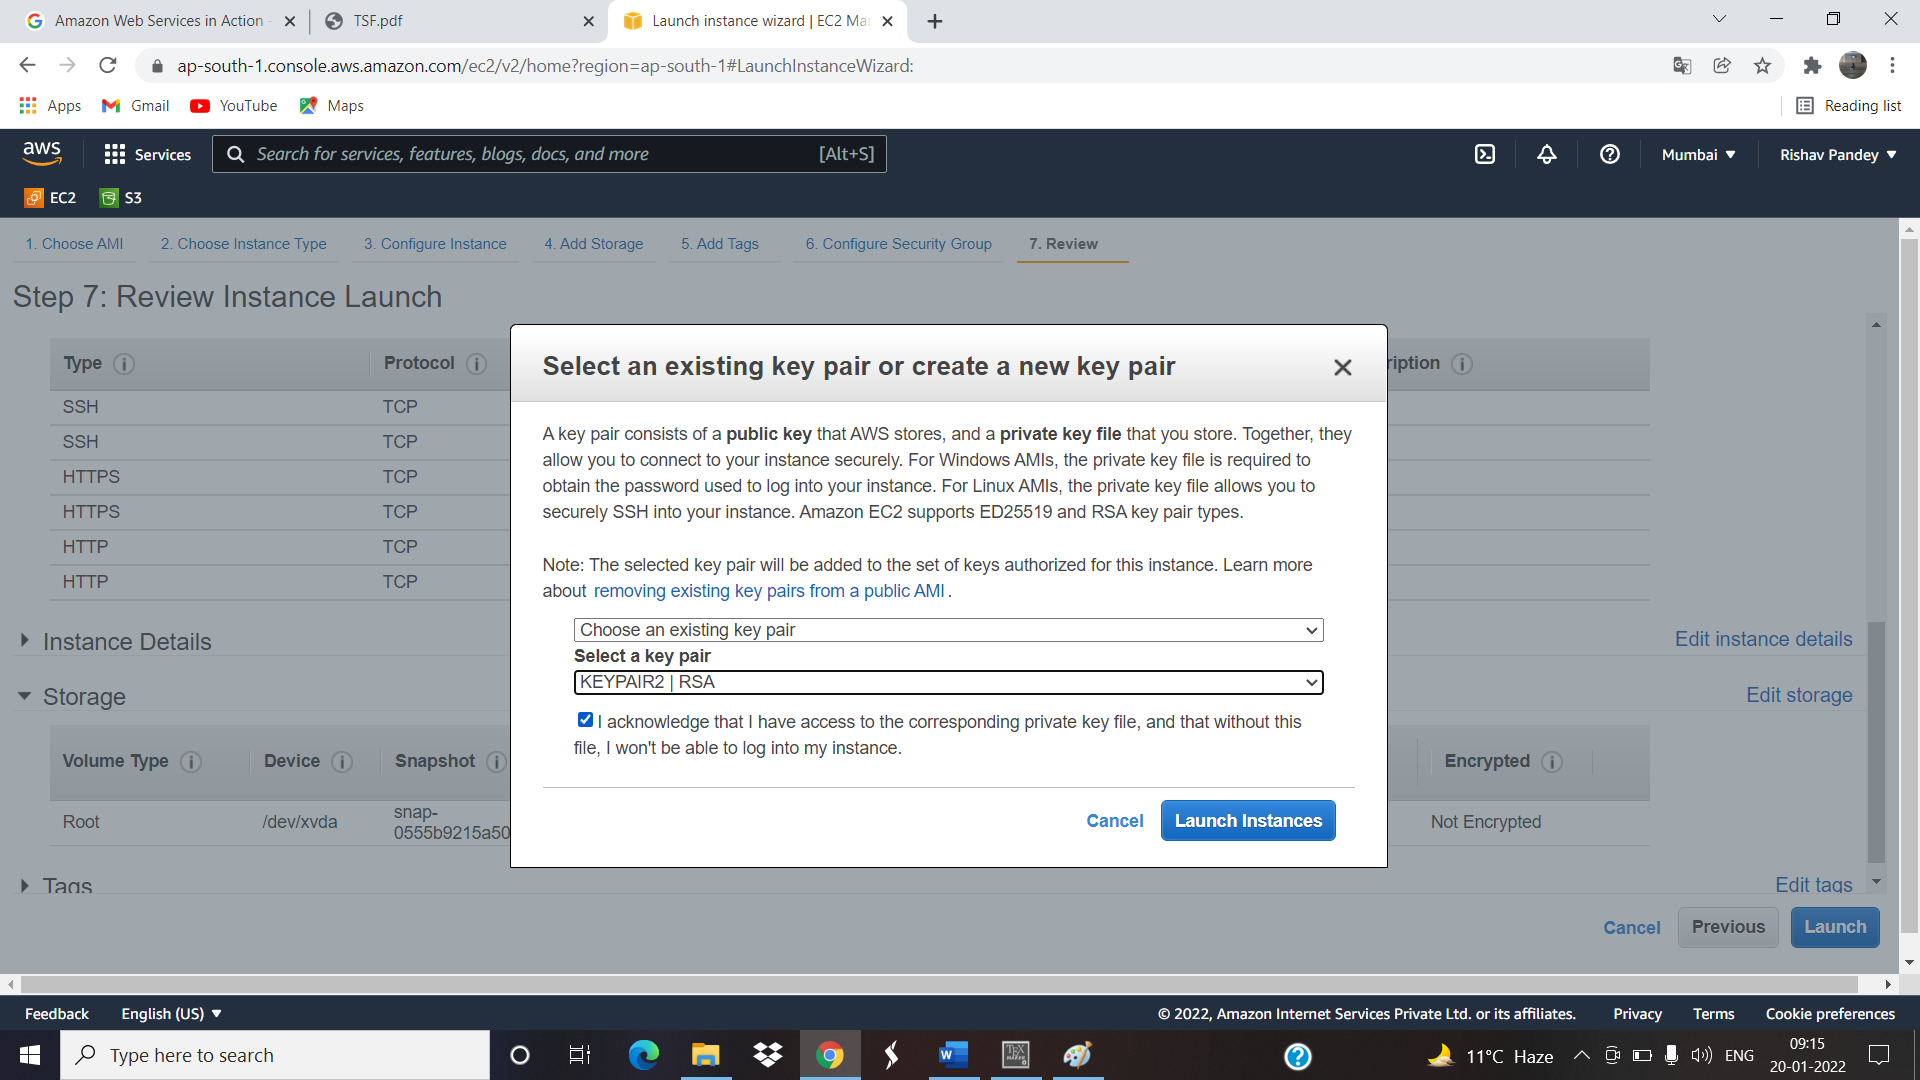
\includegraphics[scale=0.265]{Untitled13.png}
\caption{Select an existing keypair or create a new key pair}
\label{Select an existing keypair or create a new key pair}
\end{figure}

\textbf{Step 9:} Connect to instance.
\begin{figure}[h]
\centering
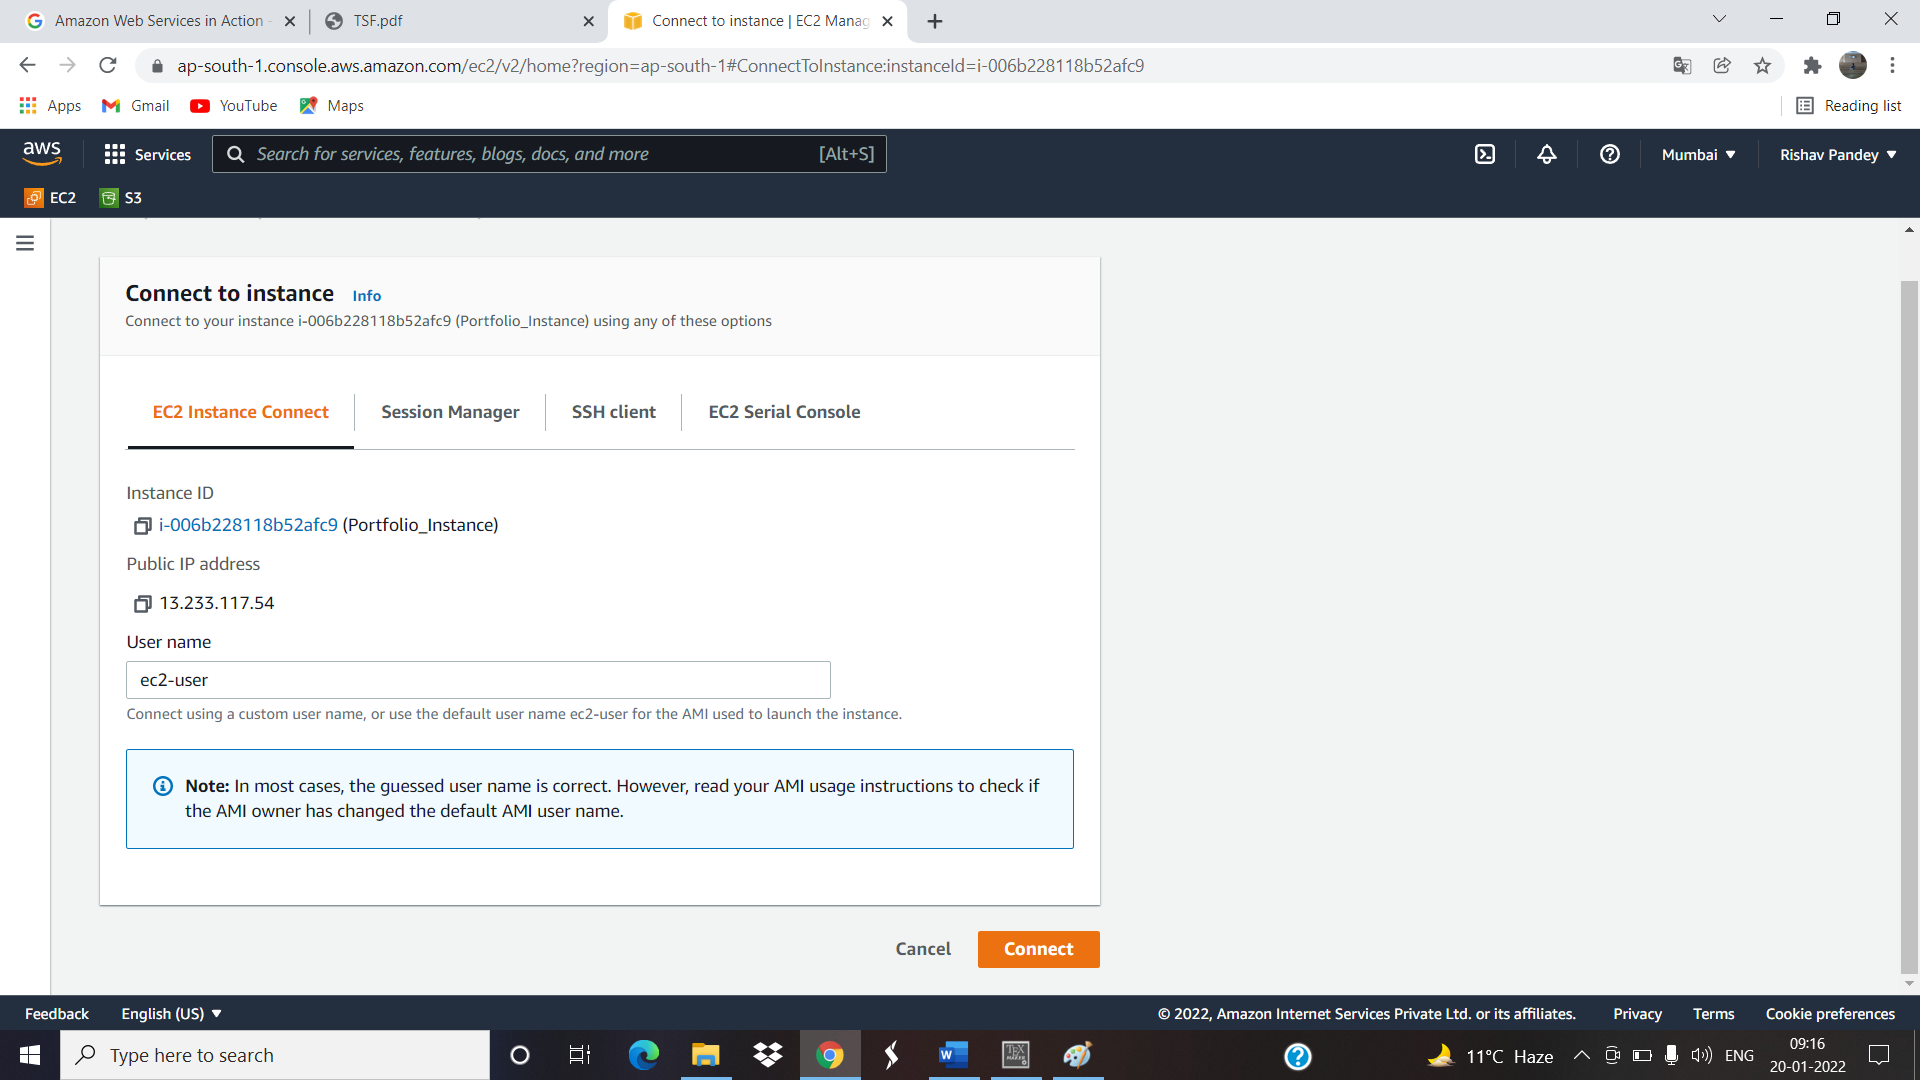
\includegraphics[scale=0.265]{Untitled14.png}
\caption{Connect to instance (i)}
\label{Connect to instance (i)}
\end{figure}
\clearpage

\begin{figure}[h]
\centering
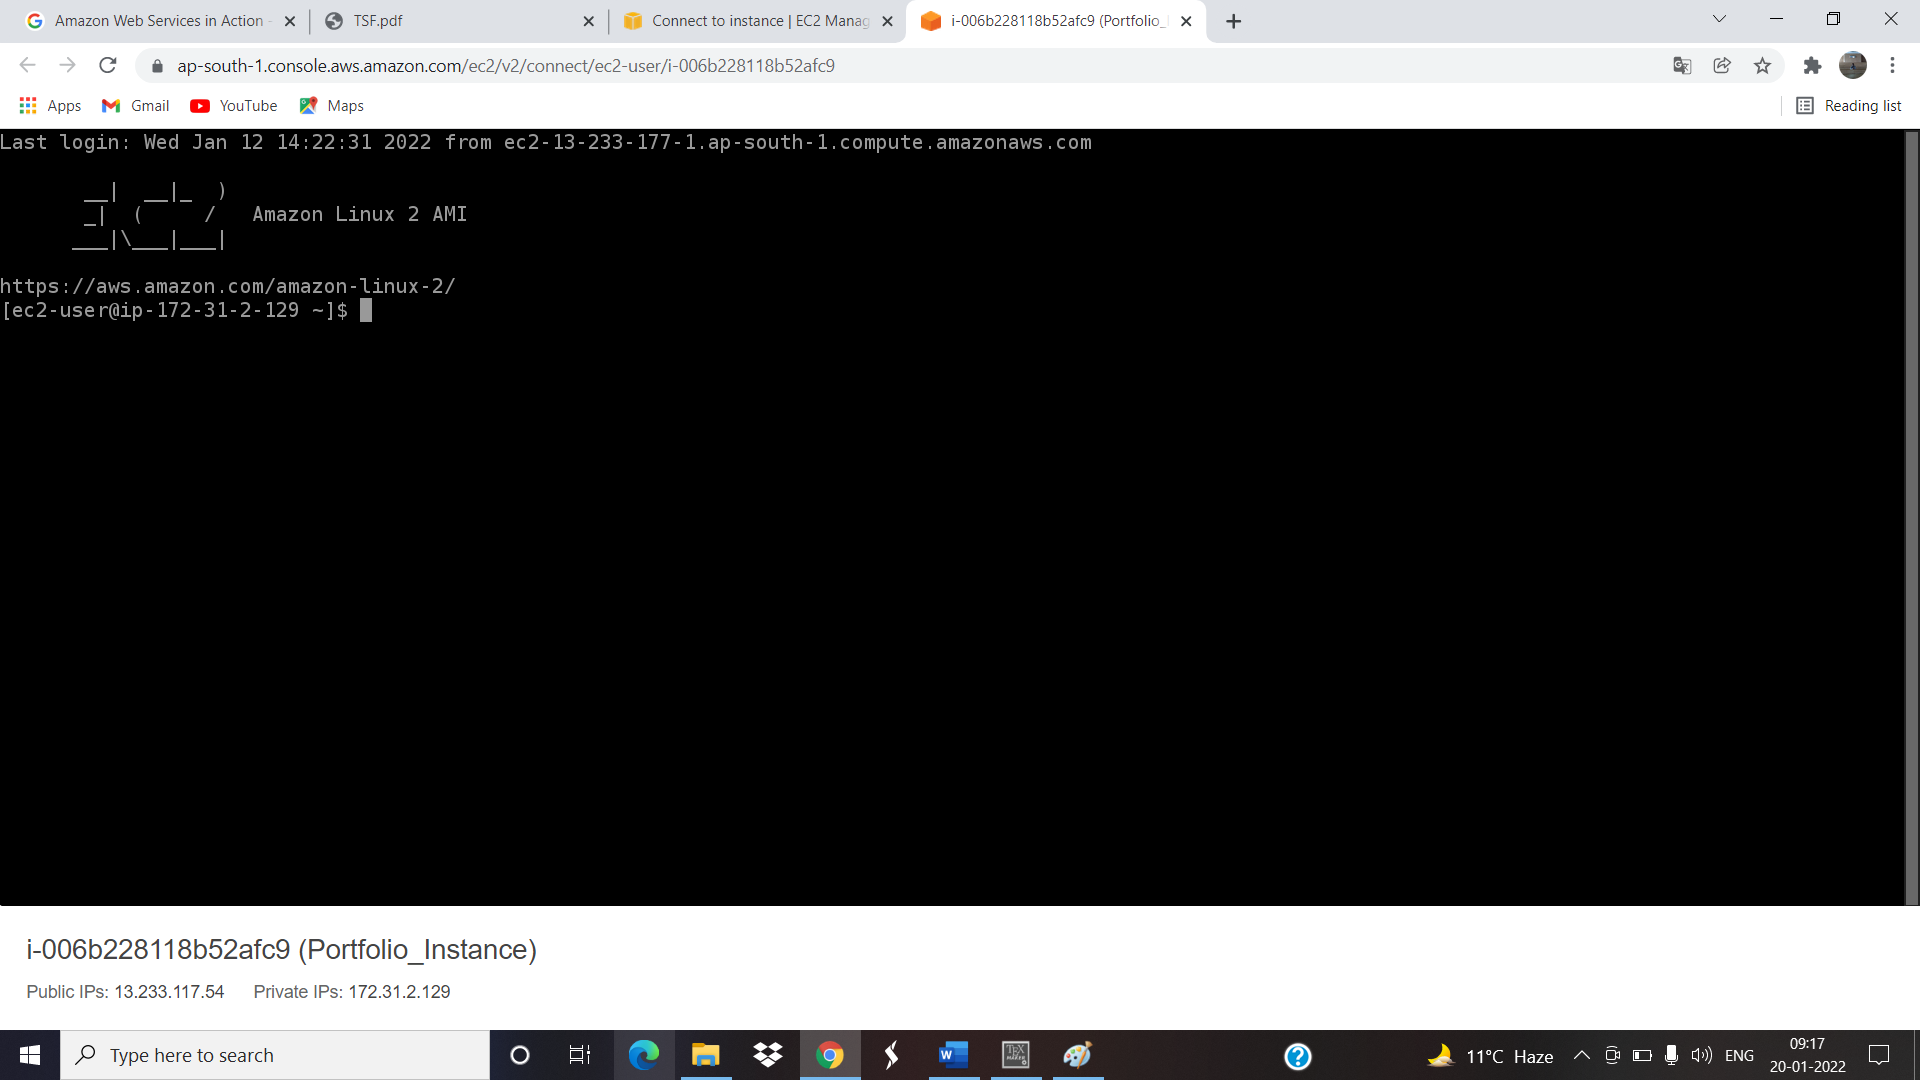
\includegraphics[scale=0.265]{Untitled15.png}
\caption{Connect to instance (ii)}
\label{Connect to instance (ii)}
\end{figure}

\textbf{Step 10:} Run the below mentioned SSH commands one by one.\\
\begin{enumerate}
\item sudo su
\item yum update -y
\item yum install httpd -y
\item chkconfig httpd on
\item cd /var/www/html
\item aws s3 sync s3://BucketName /var/www/html
\item service httpd start
\end{enumerate}
\clearpage

\begin{figure}[h]
\centering
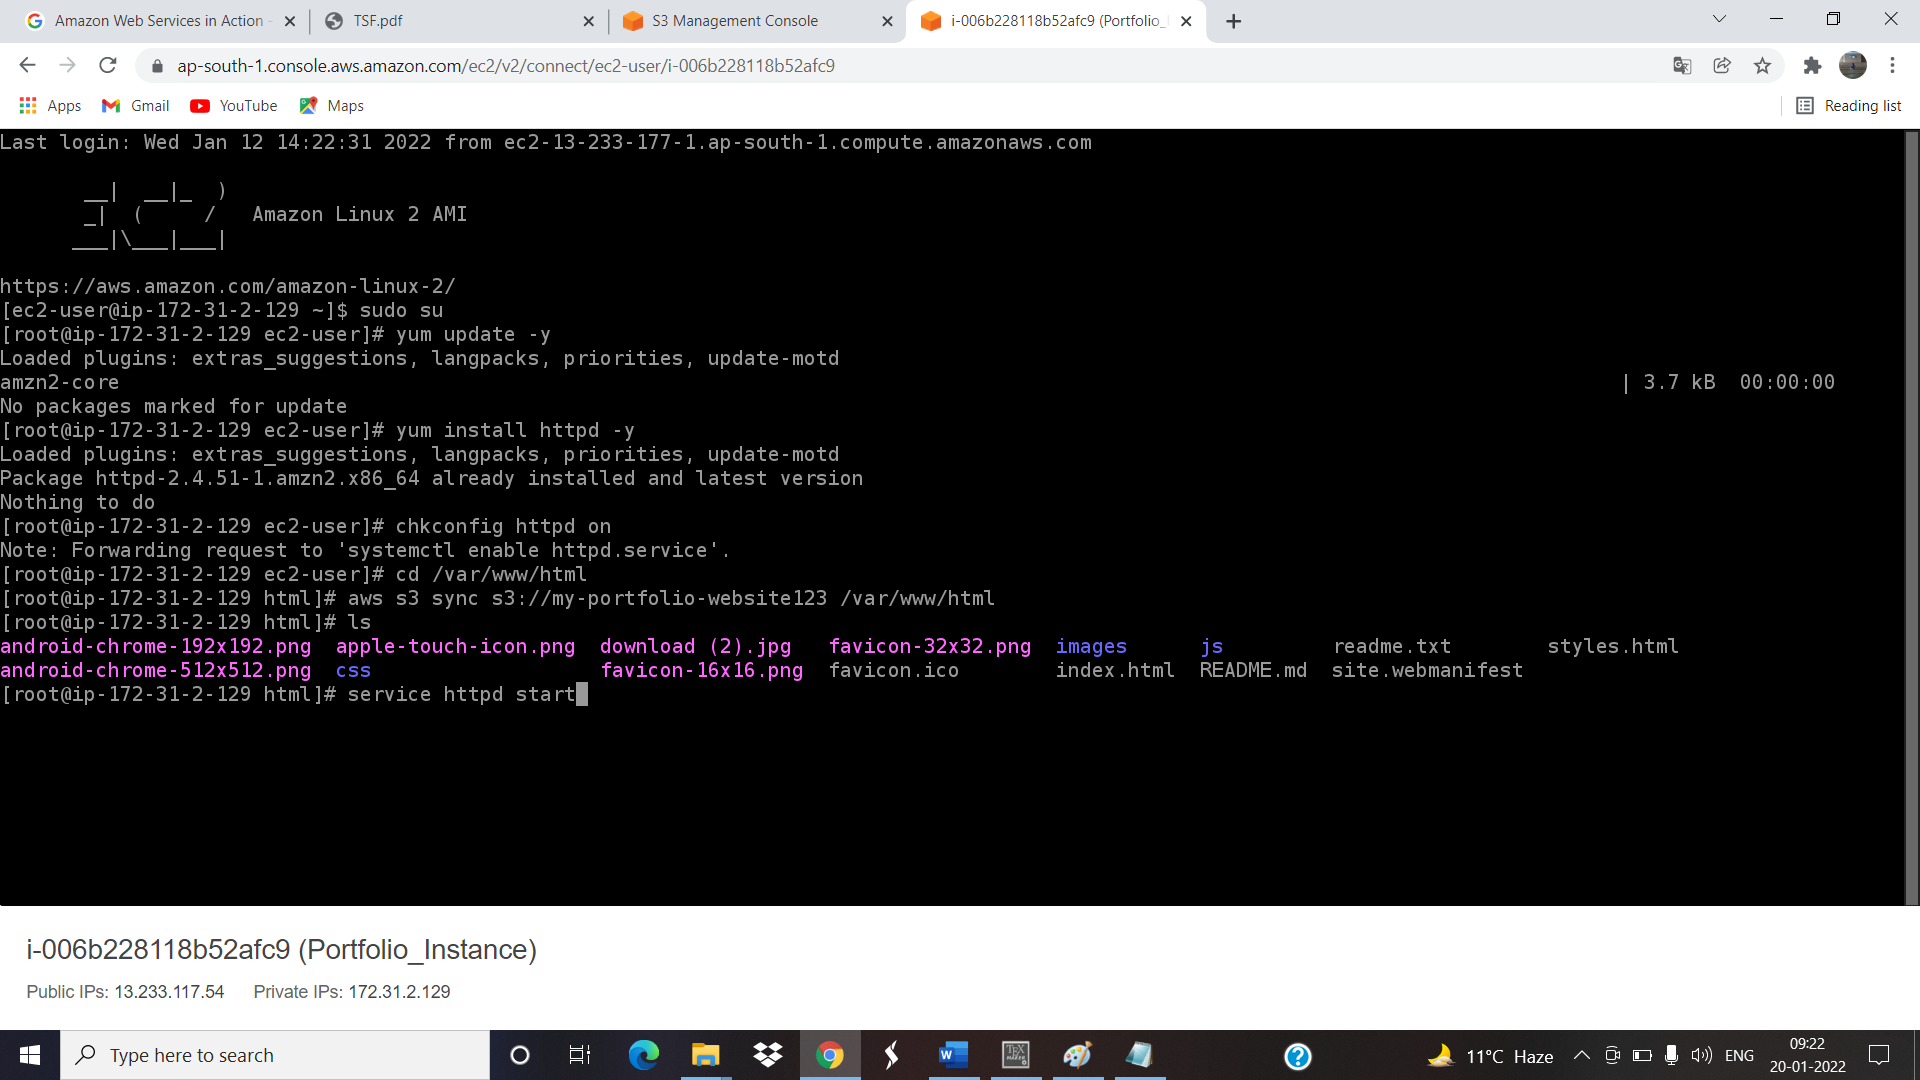
\includegraphics[scale=0.265]{Untitled16.png}
\caption{Commands being ran}
\label{Commands being ran}
\end{figure}

\textbf{Step 11:} Copy the public IPv4 address and paste it in a new tab.\\

 Your website will be live. I Just hosted my portfolio website :-)

\begin{figure}[h]
\centering

\includegraphics[scale=0.265]{Untitled17.png}
\caption{Website live on AWS EC2}
\label{Website live on AWS EC2}
\end{figure}
\clearpage


\section{Essentials of AWS EC2}
\begin{itemize}
\item \textbf{Scalability:} We can scale up or scale down the storage depending upon the traffic server. If there is a low traffic in our server then we can decrease it's storage and vice versa.\cite{varia2014overview}
\item \textbf{Flexibility:} In terms of flexibility, AWS is highly flexible. Suppose, if we want to host our website or an application for only 1 hour then we have to pay for only one hour.\cite{mishra2017amazon}
\item \textbf{Security:} AWS takes care of our stored data \& also eliminates suspicious activities.\cite{mathew2014overview}
\item \textbf{Cost Effective:} AWS has something called 'Free Tier Account' where we can use all the features of AWS free for whole one year. It also has a feature 'Pay as you go model' i.e. we have to pay only for those services which we have taken at lease.\cite{wittig2018amazon}
\end{itemize}

\href{http://13.233.117.54/}{Link of the website running on AWS EC2 Instance}\\

\href{https://github.com/rishavpandey160999/AWS-EC2-WEBSITE-HOSTING}{GitHub Repo}\\

\href{https://youtu.be/Y5yV4eJSVmc}{Presentation}



\clearpage
\bibliographystyle{apacite}
\bibliography{References}
\end{document}